\documentclass[british,titlepage]{ntnuthesis}

\title{Mosaicing of multibeam sonar feed to automate the creation of underwater sonar maps}
\shorttitle{Mosaicing FLS}
\author{Juan Pablo Pino Bravo}
\shortauthor{JPino$@$NTNU}
\date{\ntnuthesisdate}

\usepackage{float}
\usepackage{hyperref}

\addbibresource{thesis.bib}


% From https://www.overleaf.com/learn/latex/Glossaries

\makeglossaries % Prepare for adding glossary entries


\newglossaryentry{latex}
{
        name=latex,
        description={Is a mark up language specially suited for
scientific documents}
}

\newglossaryentry{bibliography}
{
        name=bibliography,
        plural=bibliographies,
        description={A list of the books referred to in a scholarly work,
typically printed as an appendix}
}

\newglossaryentry{maths}
{
    name=mathematics,
    description={Mathematics is what mathematicians do}
}


% --------------------
% ----- Acronyms -----
% --------------------


\newacronym{sonar}{SONAR}{Sound Navigation and Ranging}
\newacronym{fls}{FLS}{Forward Looking \acrshort{sonar}}
\newacronym{rov}{ROV}{Remotely Operated Vehicle}
\newacronym{bsosonar}{BSO-M1200d}{Blueprint Subsea Oculus M1200d \acrshort{fls}}
\newacronym{dvl}{DVL}{Doppler Velocity Log}
\newacronym{wldvl}{WL-A50}{WaterLinked \acrshort{dvl} A50}
\newacronym{fft}{FFT}{Fast Fourier Transform}
\newacronym{cps}{CPS}{Cross Power Spectrum}
\newacronym{dog}{DoG}{Difference of Gaussians}
\newacronym{cli}{CLI}{Command Line Interface}
\newacronym{snr}{SNR}{Signal to Noise Ratio}


\newacronym{phd}{PhD}{philosophiae doctor}
\newacronym{CoPCSE}{CoPCSE@NTNU}{Community of Practice in Computer ScienceEducation at NTNU}
\newacronym{gcd}{GCD}{Greatest Common Divisor}
 % add glossary and acronym lists before document

\begin{document}

\chapter*{Abstract}
\label{chap:abstract}

% The \texttt{ntnuthesis} document class is a customised version of the standard \LaTeX{} \texttt{report} document class. It can be used for theses at all levels – bachelor, master and PhD – and is available in English (British and American) and Norwegian (Bokmål and Nynorsk). This document is ment to serve (i) as a description of the document class, (ii) as an example of how to use it, and (iii) as a thesis template.

\chapter*{Sammendrag}

Denne oppgaven utforsker utvikling og evaluering av bilderegistreringsrørledninger for undervannsnavigasjon, spesielt ved bruk av Forward Looking SONAR (FLS) data. Utviklet i samarbeid med Blueye Robotics, fokuserer oppgaven på å bruke Fourier-baserte registreringsteknikker for å generere mosaikk fra sonarrammer og estimere odometri for Remotely Operated Vehicle (ROV). To nøkkelrørledninger analyseres: den tradisjonelle Fourier-Mellin-transformasjonen og hvordan den er tilpasset for sonarregistrering, og Fourier-basert rørledning av Hurtós et al., referert til i teksten som "Raw Polar". Gjennom testing ble det bestemt at Raw Polar Pipeline utmerker seg ved rene rotasjoner og små translasjoner over surge-aksen, mens Fourier-Mellin Pipeline er svært robust ved fjernregistrering uavhengig av rotasjon eller translasjonsretning. Selv om det ble foreslått som et raskere alternativ til Fourier-Mellin-tilnærmingen over ekkoloddrammer, ble det funnet noen problemer med Raw Polar-implementeringen som ville påvirke registreringer over svaioversettelser og i global justering. Det ble også fastslått at gitt nok ned-sampling, kan Fourier-Mellin-rørledningen overgå Raw Polar i total registreringstid. Alt i alt tyder funnene på at en rørledning som kjører i sanntid på dronen ville muliggjøre bedre navigasjon samtidig som behovet for ytterligere posisjoneringsverktøy reduseres.

\tableofcontents
\listoffigures
\listoftables
\lstlistoflistings

\printglossary[type=\acronymtype] % Print acronyms
\printglossary                    % Print glossary

\chapter{Introduction}
\label{chap:introduction}

\section{About the project}

This thesis describes and documents the author's master's project, TTK4900, on underwater navigation. It was completed in partnership with Blueye Robotics AS. TTK4900 is worth 30 credits, with a project duration of 20 full-time weeks. The work presented in this thesis is an independent effort that is supervised by Professor Annette Stahl of NTNU and Johannes Schrimpf of Blueye via frequent status meetings.

\subsection{\acrshort{sonar} imaging}

\begin{figure}[H]
  \centering
  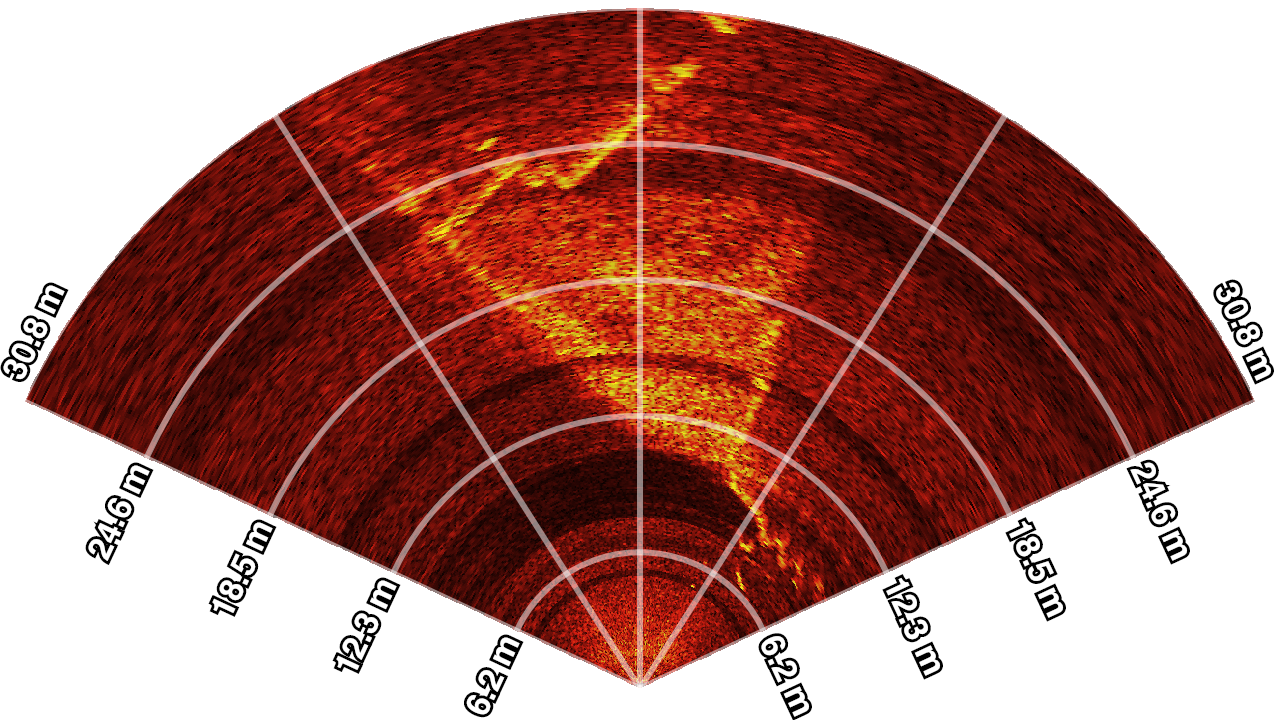
\includegraphics[width=.7\textwidth]{figures/sonar_processed.png}
  \caption[\acrshort{fls} image from \acrshort{bsosonar}]{Image obtained through a \acrfull{bsosonar} mounted on a Blueye Robotics X3 \acrshort{rov}}
  \label{fig:sonarapp}
\end{figure}

Underwater drones have revolutionized the way we explore underwater environments, providing unparalleled ease in accessing areas previously difficult to reach. However, visibility underwater is often severely limited, with cameras typically capturing images only within a few meters. To overcome this challenge, tools like \acrfull{fls}  are employed, allowing us to explore greater distances with relative ease. Despite its advantages, \acrshort{fls} is constrained by physical factors that result in noisy, inaccurate, and incomplete images, making the data difficult to interpret. From a single frame it may be very difficult to pick out useful information but given more information from a sequence of frames we can understand better what we see.

To address these challenges, image processing techniques can be applied to the frames recovered from \acrshort{fls}. Much research has gone into better visualization techniques of the covered area through mosaicing and noise reduction. And very interestingly image registration techniques may also allow for the estimation of the drone’s movement. In this thesis, I will implement an image processing pipeline that creates a mosaic of all the image frames and estimates odometry using data collected from a \acrfull{rov} equipped with \acrshort{fls}. This approach aims to enhance the clarity and usability of the \acrshort{sonar} data, ultimately improving the ability to navigate and understand underwater environments. If successfully implemented in real-time, the benefits to navigation using an \acrfull{rov} would be great. 

\section{The Project Proposal - Mosaicing \acrshort{fls} frames to aid in \acrshort{rov} navigation}

\begin{figure}[H]
  \centering
  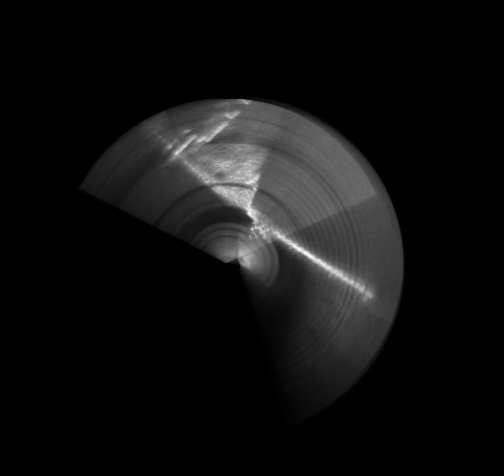
\includegraphics[width=.7\textwidth]{figures/example-output.png}
  \caption[Example mosaicing]{Mosaicing of \acrshort{bsosonar} frames captured on Blueye \acrshort{rov}}
  \label{fig:sonarapp}
\end{figure}

Being the product of collaboration with Blueye Robotics, the ultimate goal of the thesis is to make the \acrshort{sonar} data collected through the drone more useful. Together with Johanness Schrimpf and Jonas Follesoe from Blueye, we've identified registration and mosaicing of \acrshort{sonar} frames as a useful feature as in the future it might unlock some other applications:

\begin{itemize}
    \item Having a map of the areas covered with the drone to refer to might aid in navigation, exploration, and reporting.
    \item Being able to visualize things beyond the range of the \acrshort{sonar} all together in one image might make inspections easier.
    \item Could turn the \acrshort{fls} into a tool for bathymetry surveys, adding more functionality to existing tools on the drone.
    \item The transformations that describe the movement between one frame and the next one are also an indication of real movement of the drone. This odometry estimation might be useful for navigation and station keeping.
\end{itemize}

\subsection{Identified Tasks}
To meet the base goal of registering image pairs and generating \acrshort{sonar} mosaics certain tasks and goals must be met:

\begin{enumerate}
    \item Gather data for testing
        \begin{itemize}
            \item Generate fake data in a similar format to the \acrshort{sonar}
            \item Capture real data using an \acrshort{fls} mounted on a Blueye \acrshort{rov}
        \end{itemize}
    \item Process raw sensor data into \acrshort{sonar} images
    \item Implement a pipeline for image registration
        \begin{itemize}
            \item Compare different approaches to image registration
        \end{itemize}
    \item Implement an image stitching step that combines the images into a \acrshort{sonar} map
    \item Compare performance of different pipelines experimentally
\end{enumerate}

\section{Contributions}

After working on this thesis these are some of my contributions to the field:
\begin{itemize}
    \item Developing a flexible image registration pipeline framework.
    \item Developing a \acrshort{cli} application to generate seabed mosaics.
    \item Proposing improvements for a combined pipeline that might take advantage of the strengths of each of the pipelines proposed in the document. 
\end{itemize}


\section{Sustainability}

Some sustainability aspects that this thesis might have an impact on:

\begin{itemize}
    \item Reduce danger for divers: by being able to map the seabed, if there is a need to send down divers, they will have more data available to make more informed decisions about their dive beforehand.
    \item Reduce the need for additional positioning equipment on the drone: this work lays the bases for future development on the drone to be able to use the sonar as a positioning system. In lieu of a \acrshort{dvl}, the sonar could be used for station keeping or dead-reckoning. Additional work is required to get this operational, assuming fast enough computing on the drone to do this in real time. 
\end{itemize}


\section{Thesis Structure}

The following chapters of the thesis will be organized as follows:

\begin{itemize}
    \item \textbf{Chapter \ref{chap:background}}: introduces background theory necessary to understand \acrshort{fls}, it's image formation process, and theory behind registration pipelines.
    \item \textbf{Chapter \ref{chap:implementation}}: delves into the actual implementation of the pipeline and its sub-modules.
    \item \textbf{Chapter \ref{chap:setup}}: explains the experimental setup and preparation of the experiments for performance comparison.
    \item \textbf{Chapter \ref{chap:results}}: presents the results of the experiments to make it easier to compare the different pipelines.
    \item \textbf{Chapter \ref{chap:discussion}}: the discussion chapter contains an assessment of the results and implementations
    \item \textbf{Chapter \ref{chap:conclusion}}: the last chapter will demonstrate how successfully the objectives of the thesis are met. It concludes with a summary of the final results and recommendations for further work.
\end{itemize}

\section{Implementation overview}

\subsection{Tools and equipment}

A Blueye Robotics X3 \acrshort{rov} was provided by the company for the project's experiments. It comes equipped with a \acrfull{bsosonar} and a \acrfull{wldvl}. The \acrshort{bsosonar} is mounted on a skid that allows for tilt through a servo. The \acrshort{wldvl} allows the drone to maintain it's position in the water using the station-keeping mode while simultaneously providing dead-reckoning based positioning of the drone.

\begin{figure}[H]
  \centering
  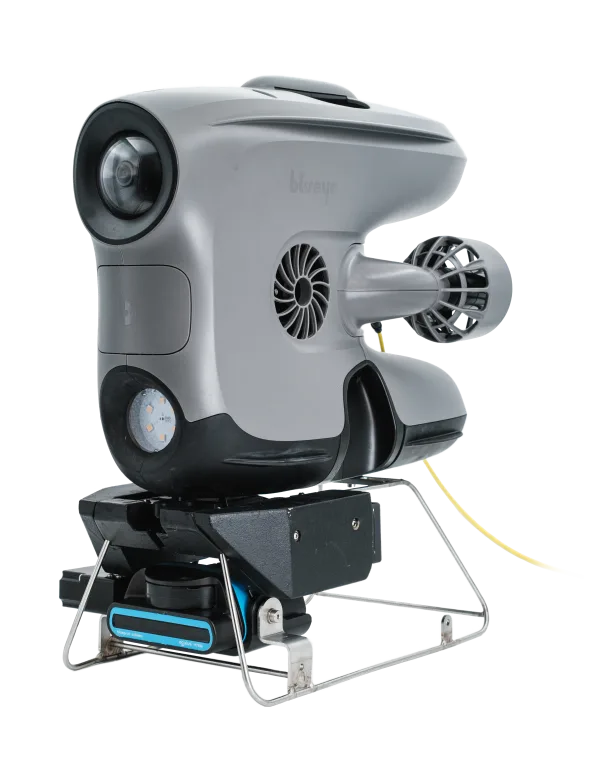
\includegraphics[width=.5\textwidth]{figures/blueye_x3.png}
  \caption[Blueye Robotics X3 \acrshort{rov} equipped with \acrshort{bsosonar}]{Equipment for experimentation provided by Blueye Robotics. Standard Blueye X3 drone equipped with a \acrshort{fls} and a \acrshort{dvl}. Image provided by Blueye \cite{Blueye:X3}.}
  \label{fig:sonarapp}
\end{figure}

On the software side, for ease of development the project uses Python as the main programming language, with extensive use of \href{https://numpy.org}{NumPy}, \href{https://scikit-image.org}{scikit-image} and \href{https://scipy.org}{scipy} for image processing and the implementation of the pipelines. In addition \href{https://www.ray.io}{Ray} is used for basic CPU parallelization. 


\chapter{Background Information and Literature}
\label{chap:background}

This chapter will introduce the necessary theory to understand \acrshort{fls}, its image formation process, and some \acrshort{fls} based approaches to registration.  

\section{Sonar Image Formation}

As is well explained by \citeauthor{noaaExplorationTools}\cite{noaaExplorationTools} and \citeauthor{Hurtos2015}\cite{Hurtos2015}, \acrfull{sonar}, sometimes also referred to as acoustic imaging, generate images using underwater sound waves. The \acrshort{sonar} contains in it an array of transducers that produce beams of acoustic waves in the water at different angles (bearings) and measure the time for it to "ping" or "echo" back. These sound waves travel across the water, reflecting off items like the bottom, underwater structures, and marine life. With this timing information, the system can generate detailed photos of the underwater world. This technology is widely utilized for navigation, mapping, and exploration, giving vital data for maritime research, underwater construction, and search and rescue operations.

Despite all of it's benefits and advantages, \acrshort{sonar} has a few pitfalls that specifically affect the goals of this thesis: 
\begin{itemize}
    \item According to \citeauthor{Hurtos2015}\cite{Hurtos2015}, the resulting images are often of low resolution, as compared to current camera technology. This is often a limitation of the medium as sound waves have a much higher wavelength than light. Higher-resolution images would offer more information and probably better-defined edges or areas of interest that would help the registration process.
    \item According to \citeauthor{Huang2020}\cite{Huang2020} sonar images tend to suffer from speckle noise: scattering and reverberation of the acoustic waves traveling through water results in a granular interference pattern that's typical of \acrshort{sonar} imaging. This is evidenced in the dark and bright spots often plaguing the image. Noise will undoubtedly introduce errors in the measurements, introducing uncertainty to the registrations. 
    \item It is susceptible to interference from other sources. For example, the onboard \acrshort{dvl} uses acoustic beams to measure the velocity of the vehicle relative to the seafloor, which can create signal interference with the sonar system, potentially leading to degraded image quality or inaccurate data. This interference might lead to inaccurate registrations which might affect the resulting output image.
\end{itemize}


The number of beams produced by the sonar and their orientation will determine the sonar's angular resolution and field of view:
\begin{figure}[H]
    \centering
    \begin{subfigure}[b]{.35\textwidth}
        \centering
        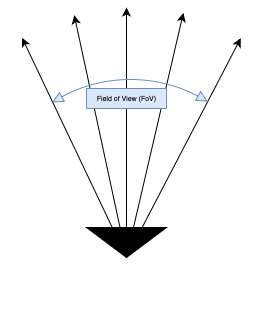
\includegraphics[width=\textwidth]{figures/FLS-TopView.png}
        \caption{Top-view of the sonar showing how all the beams spread out from the device.}
        \label{fig:flstop}
    \end{subfigure}
    \hfill
    \begin{subfigure}[b]{.55\textwidth}
        \centering
        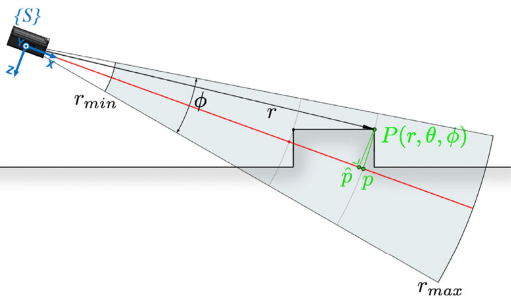
\includegraphics[width=\textwidth]{figures/FLS.png}
        \caption{Side-view of the sonar showing the effect of the \acrshort{fls} vertical aperture. Image created by \citeauthor{Hurtos2015} \cite{Hurtos2015}.}
        \label{fig:flsaperture}
    \end{subfigure}
    \caption{Top and side views of the sonar beams. In the side-view image, only one beam coming from the sonar is shown.}
\end{figure}


As explained by \cite{Hurtos2015}, in \acrfull{fls} imaging, a particular beam generated from the transducer might spread along its "Vertical Aperture". All the pings along the aperture arc get compacted down into the image plane. In a similar fashion to what happens in a regular optical camera, a 2D \acrfull{fls} loses 3D information of the captured scene. Any set of points above or below the image plane along the same arc will correspond to the same output in the sonar image. The figure \ref{fig:flsaperture} shows a single beam coming from the sonar and how it is mapped into a single vertical line in the output image. Any echoes received back from insonifying this cone will be mapped onto the red "imaging plane", generating the loss of 3D data. 

Although the 3D point \(P\) actually matches the point \(p\) on the imaging plane, as long as the range is much greater than the relief observed in the elevation direction we can approximate the 3D point \(P\) to \(\hat{p}\). This is often the case as on \acrshort{fls} the vertical aperture tends to be small, and ranges can extend very far.


\subsection{Fan Transformation}
\label{sec:fan-tform}
\begin{figure}[H]
    \centering
    \begin{subfigure}[b]{.45\textwidth}
        \centering
        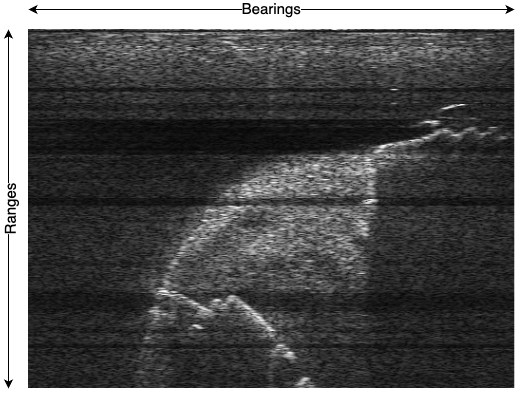
\includegraphics[width=\textwidth]{figures/sonar_raw_annotated.png}
        \caption[\acrshort{fls} raw data]{Raw data obtained from the sonar}
        \label{sfig:sonarraw}
    \end{subfigure}
    \hfill
    \begin{subfigure}[b]{.45\textwidth}
        \centering
        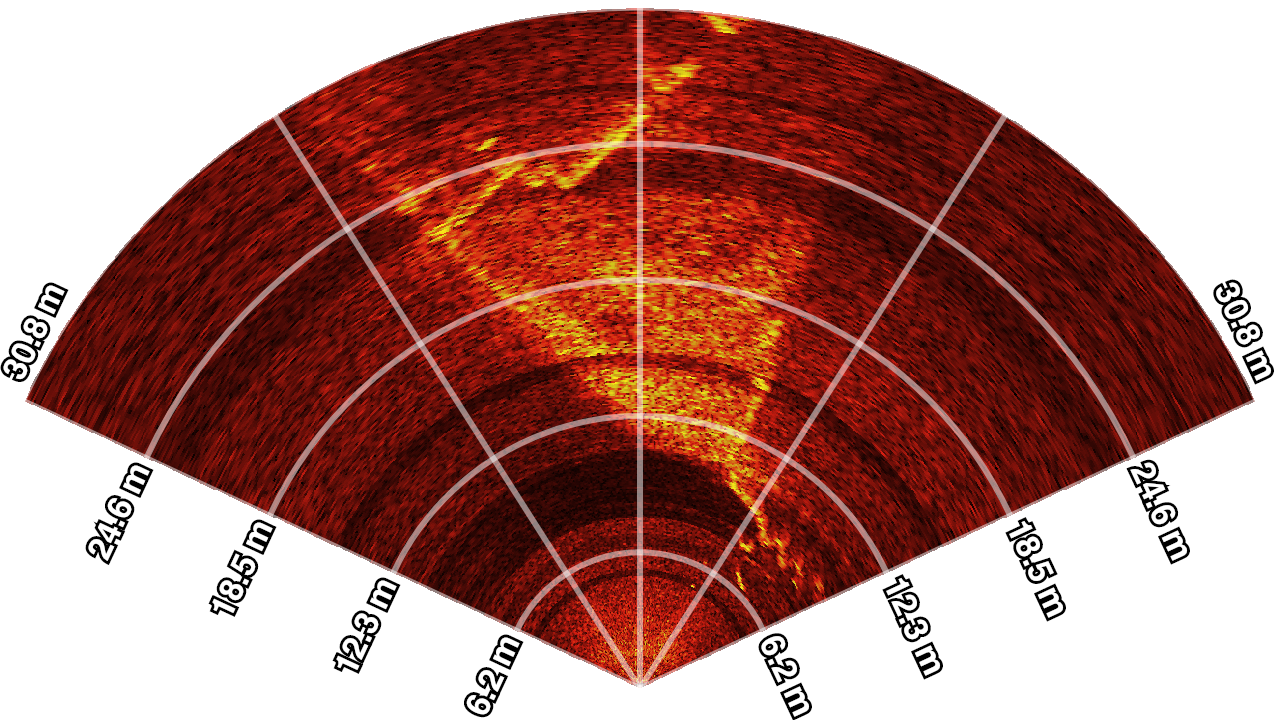
\includegraphics[width=\textwidth]{figures/sonar_processed.png}
        \caption{Processed \acrshort{fls} data}
        \label{sfig:sonarfan}
    \end{subfigure}
    \caption{Using the data from the bearing table we can transform the raw data into actual sonar images.}
\end{figure}

From the sonar driver code and its resources \cite{Blueye:OculusDriver} a few things become clear. The raw data from the sensor is structured in an array that represents ping intensity at a specific bearing and range. It is important to note that the beam bearings are not evenly spaced. The sensor provides a bearing table that accompanies the frame with the specific angle associated with each beam. Using this information we can create a mapping \(F(u,v)=I(\theta,r)\) that will produce pixel values for the output fan image based on the bearing and range from the source image. For any \((u,v)\) pair in the output fan image, we can calculate the corresponding \((\theta, r)\) from the source image. Looking only at the output image, we see that the mapping from \((\theta, r)\) to \((u, v)\) boils down to simple trigonometry. The output image will have the same height (\(H\)) as the input image, i.e. the number of ranges. The width will be limited by the maximum and minimum bearing angle and the height of the image. It can be calculated as follows: 

\begin{equation}
    W = 2 * H * \sin{\frac{FOV}{2}} 
\end{equation}

There are a couple of considerations to keep in mind:
\begin{itemize}
    \item The top row of the raw image \ref{sfig:sonarraw} has index 0. Since the output image \ref{sfig:sonarfan} expects the origin of the rays to be at the bottom, the image must be flipped. This can be achieved by replacing the y-coordinate \(v\) with \(H - v\), where \(H\) is the height of the images (the number of ranges).
    \item The angle \(\theta\) is measured between the beam in question and the y-axis of the output fan image. This axis is centered in the image as in \ref{sfig:sonarfan}. To center the coordinate frame, the x-coordinate \(u\) is replaced with \((u - W / 2)\), where W is the width of the output image.
    \item Any mapping that results in a value of \(r\) beyond the number or ranges in the source image is invalid, i.e. \(r \in [ 0, maxRange ]\). The same goes for values of theta that are outside of the range of the bearing table, i.e. \(\theta \in [ -minBearing, maxBearing] \). In any of these cases, the resulting pixel will be outside of the fan.
\end{itemize}


\[
\theta = \arctan(\frac{u - W / 2}{ H - v}))
\]
\[
r = \sqrt{(u - W / 2) ^ 2 + (H - v)^ 2}
\]

The value of \(r\) will represent then the y-axis coordinate in the source image (the "Ranges" axis). It is necessary to round it to the closest integer to access the pixel value. The value of \(\theta\) can be linked to its corresponding index along the x-axis of the source image through the bearing table. The index of the closest value to \(\theta\) will represent the coordinate on the "Bearings" axis.

\section{Speedup}
\label{sec:speedup}

Speedup is a metric that will be used to evaluate some of the results. It is a measure of the relative performance of two systems evaluating the same problem \cite{enwiki:1225834080}:

\[S_{latency} = \frac{L_{old}}{L_{new}}\]


\section{Mosaicing}
\label{sec:mosaicing}


According to \citeauthor{Capel2001}\cite{Capel2001}:
\begin{quote}
\textit{Image mosaicing is the alignment of multiple images into larger compositions which represent portions of a 3D scene. It generally applies to images related by planar homographies.}
\end{quote}

According to \citeauthor{Capel2001}, homographies can be estimated from images in two cases:
\begin{itemize}
    \item \textbf{Images of planes:} images taken from different viewpoints of a fully planar surface.
    \item \textbf{Rotation about the camera center}: images taken as the camera rotates about its center. The scene is allowed to be 3D in this case.
\end{itemize}

If the range that the sonar images are taken from is much larger than whatever variation in depth there is at the seabed, we can approximate our system as taking images of a planar surface in which case traditional mosaicing techniques would apply. 

Using the techniques that will be described in the following sections it will be possible to estimate these homographies between consecutive frames. What's left after that is implementing an algorithm that would combine the data from all the frames using the estimated homographies.

Combining the images is a topic in itself. There are many considerations like the best way to blend the seams, the best way to reduce noise, super-sampling, etc. A simple approach, but quite effective against speckle noise is averaging the overlapping part of the images. Since the noise and the underlying signal have a low correlation, averaging the images results in a noise-attenuating effect. Ideally, this reduction of noise is proportional to the squared number of average samples \cite{Hurtos2015}. For example, to cut the noise in half in the area of the mosaic, four overlapping images would be required. 
% \section{\acrfull{dvl}}

\section{Registration in the Frequency Domain}

"Registration in the frequency domain" describes methods that often use the Fourier transform to estimate the transformation between two images. They are often based on properties of the \acrfull{fft}, and offer several advantages that are of interest to the registration of sonar images:
\begin{itemize}
    \item Robustness to noise: Frequency domain methods, especially when using phase correlation, are relatively robust to noise and intensity variations\cite{Reddy1996}.
    \item Frequency domain methods can be extended to handle not just translations, but also rotations and scaling \cite{Reddy1996}.
    \item Low computational complexity of the \acrshort{fft}:  \(O(N\log_2N)\)\cite{Haynal2011}. Fast and inexpensive methods are preferred so as to not restrict where the algorithm might run. This could allow the \acrshort{rov} to execute the algorithm on a much more limited CPU.
\end{itemize}

Robustness to noise in particular is of interest when developing registration pipelines for sonar images. As mentioned before, sonar images are very noisy. Feature-based algorithms might mistake the noise as relevant image information which would be undesirable.

\subsection{Phase Correlation}

The phase correlation method allows us to estimate translations between images using the Fourier transform. By converting the images into the frequency domain, the method identifies shifts as phase differences between their corresponding Fourier transforms. The resulting phase correlation peak indicates the relative translation between the images, providing a robust and efficient way to align them even in the presence of noise or varying image intensities. It uses a property called Fourier shift which relates translations in the spatial domain to phase shifts in the Fourier domain. 


Better explained by \citeauthor{Reddy1996}\cite{Reddy1996}, the process of identifying the translation between two images is as follows. Given two images \(f_1\) and \(f_2\) related by a translation in the x and y axis, \(t_x\) and \(t_y\) respectively:

\[f_2(x,y)=f_1(x-t_x,y-t_y)\]

When converted to the Fourier domain:

\[F_2(\xi,\eta)=e^{-j2\pi(\xi t_x + \eta t_y)} F_1(\xi,\eta)\]

It can be concluded that the Fourier transform of each image is the same in magnitude, but has a phase shift given by \(e^{-j2\pi(\xi t_x + \eta t_y)}\). The shift theorem guarantees that the phase of the cross-power spectrum is equivalent to the phase difference between the images. Using the normalized \acrfull{cps} we can calculate this phase shift:

\[e^{-j2\pi(\xi t_x + \eta t_y)} = \frac{F_1(\xi,\eta) \; F_2^*(\xi,\eta)}{|F_1(\xi,\eta) \; F_2(\xi,\eta)|}\]

Computing the inverse Fourier transform of the \acrshort{cps} returns an impulse function, i.e. mostly zeros everywhere except for a peak/impulse. This is also called a dirac delta function. The coordinates of this peak represent the shifts \(t_x\) and \(t_y\).

Although this is a great building block for the registration pipeline, it has the limitation of only being able to detect translations. The images that will be captured in the sonar will also experience rotations which makes this method, by its own, useless. This is where the next point, the polar and log-polar transforms come in.

\subsection{Polar Transforms}

The polar transform in this context is used to to convert from a 2D cartesian coordinate system to 2D polar coordinate system. Coordinates typically expressed in \((x, y)\), are represented by radius and angle \((\rho, \theta)\) as measured from the image center \((x_x, y_c)\):

\[\rho = \sqrt{(x-x_c)^2 + (y - y_c)^2}\]
\[\theta = \arctan{\frac{y - y_c}{x-x_c}}\]

This brings rise to a useful property: rotations in the cartesian coordinate system are represented by shifts in the $\theta$ axis of its polar counterpart.

Recalling the structure of the images provided by the sonar, this sounds very familiar. Indeed, the raw sonar frames are a polar representation of the scene. 

There is still one more issue that a regular polar transform can't account for: scaling of the images. According to \citeauthor{5396234}\cite{5396234}, in a log-polar transform scaling is represented by a shift in the $\rho$ axis:

\[\rho = \log(\sqrt{(x-x_c)^2 + (y - y_c)^2}\]
\[\theta = \arctan{\frac{y - y_c}{x-x_c}}\]

Knowing that we can use phase correlation to identify translations in images, a combination of a polar transform and phase correlation might help us then identify the rotation between the images. This is what the Fourier-Mellin approach proposes.

\section{Fourier-Mellin Registration Pipeline}
\label{sec:fm-registration}

The Fourier-Mellin registration pipeline takes advantage of a second property of the Fourier transform of two images in the case when they are rotated. Again \citeauthor{Reddy1996}\cite{Reddy1996} explains it in simple terms. Given two images \(f_1\) and \(f_2\) related by a translation \(t_x\) and \(t_y\) and a rotatation \(\theta\):

\[f_2(x,y)=f_1(x \cos{\theta} + y \sin{\theta} -t_x, - x \sin{\theta} + y \cos{\theta} - t_y)\]

When converted to the Fourier domain:

\[F_2(\xi,\eta)=e^{-j2\pi(\xi t_x + \eta t_y)} F_1(\xi\cos{\theta} + \eta\sin{\theta},-\xi\sin{\theta} + \eta\cos{\theta})\]

Ignoring the phase and only working with the polar representation of the magnitudes, rotational movement \(\theta_0\) decoupled from translations can be deduced by using phase correlation.

\[M_2(\xi,\eta)=M_1(\xi\cos{\theta} + \eta\sin{\theta},-\xi\sin{\theta} + \eta\cos{\theta})\]
\[\mbox{Converting to polar representation, }M_2(\rho,\theta)=M_1(\rho,\theta - \theta_0)\]
\[\mbox{Applying phase correlation and identifying peak} \rightarrow \theta_0\]

This can be extended to account for scaling differences using the log-polar transform. This process is also used by \citeauthor{5396234}\cite{5396234} to register medical images, which are generated in a similar fashion to sonar. In this case, when applying phase correlation, the coordinates of the peak will represent both scaling and rotation.

In essence the Fourier-Mellin Pipeline does the following:

\begin{itemize}
    \item Apply the Discrete Fourier Transform (DFT) to shift images into the frequency domain.
    \item Use smoothing and high-pass filtering to prevent border-induced artifacts and reduce aliasing artifacts caused by rotation.
    \item Perform a log-polar transform to map rotation and scaling in Cartesian coordinates to translations in the log-polar coordinate system.
    \item Use Phase Correlation to determine the translation offset between two images. This yields rotation.
    \item Apply this rotation to the original image.
    \item Use Phase Correlation again over the rotated image to identify translation.
\end{itemize}

The most attractive factor of this approach is that it can decouple the rotation of the image from its translation. On simulated data, it is possible to achieve perfect rotations and perfect translations, but when using data from a sonar mounted to the \acrshort{rov}, the frames will experience both rotation and translation at the same time from the smallest perturbations, even if the sonar is trying not to move, or trying to only rotate or translate in one direction.


\section{\citeauthor{Hurtos2015}'s Raw Polar Registration Pipeline}

\begin{figure}[H]
  \centering
  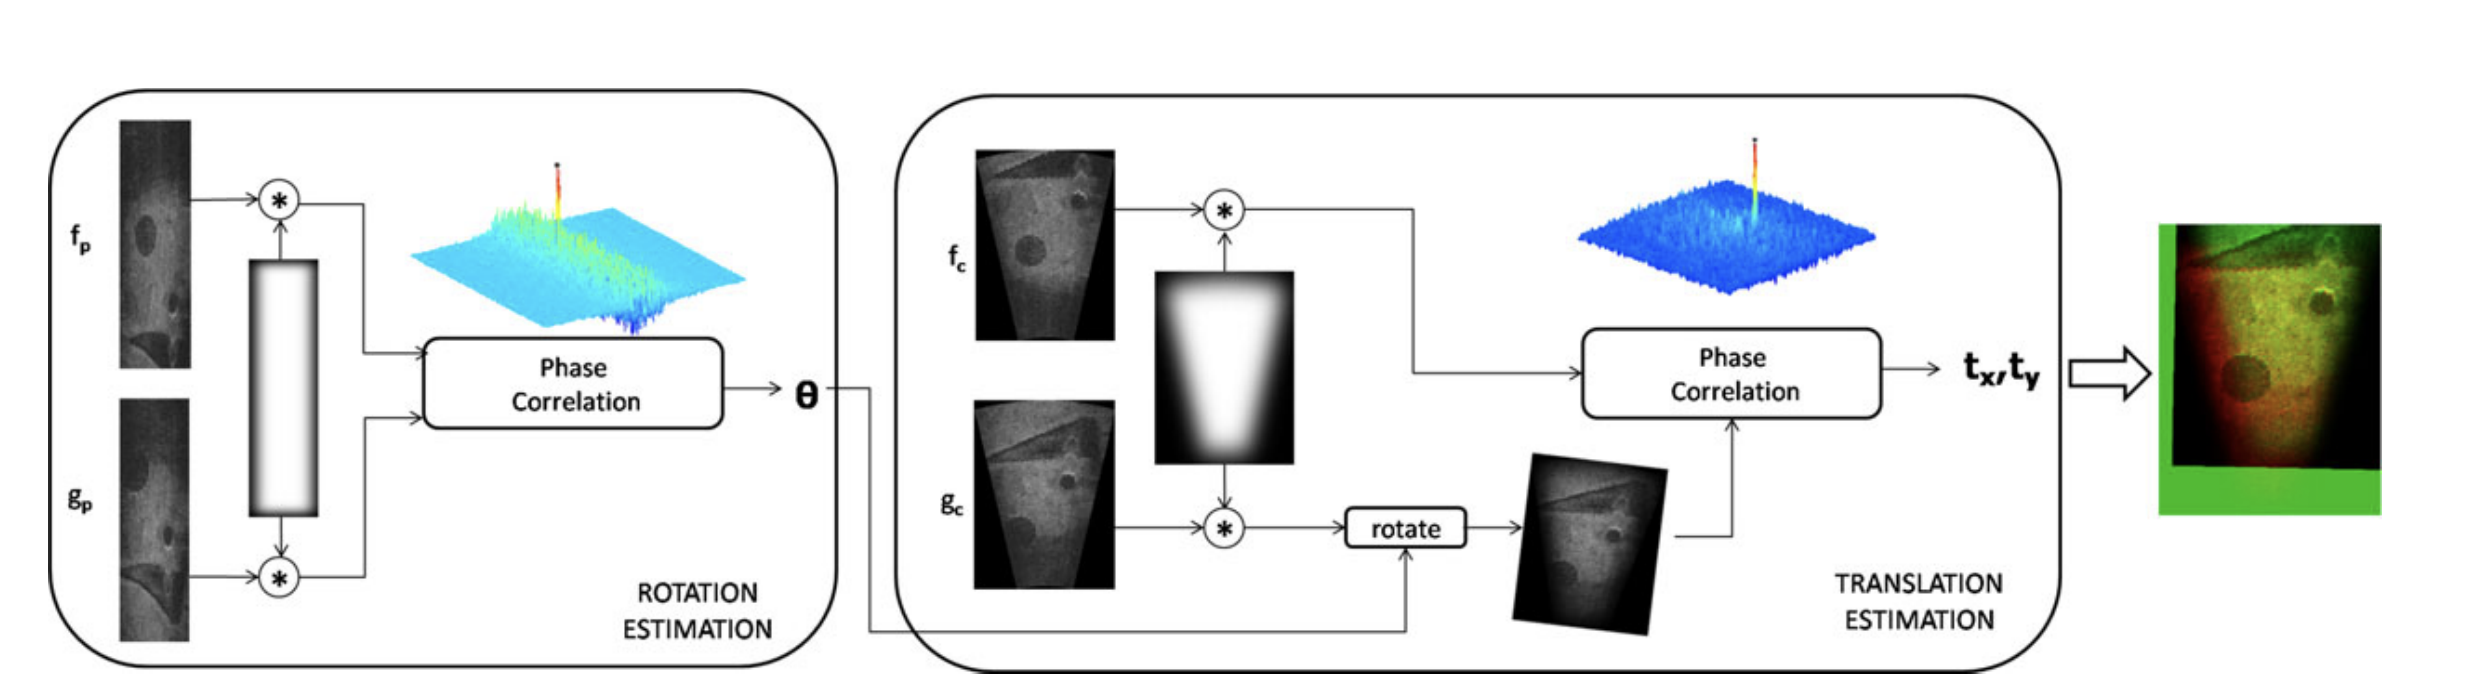
\includegraphics[width=\textwidth]{figures/RawPolarPipeline.png}
  \caption{Raw Polar Registration Pieline. Image created by \citeauthor{Hurtos2015}\cite{Hurtos2015}.}
  \label{fig:raw-polar-pipeline}
\end{figure}


\citeauthor{Hurtos2015} proposes a shorter pipeline than the Fourier-Mellin approach. Instead of estimating the rotation using the Log-Polar transform of the images in Fourier domain, it proposes using Phase Correlation over the raw sonar frames. Because of this, the pipeline will be referred to through the text as the "Raw Polar Pipeline". Since the input frames are already in a polar representation of sorts, given a short enough displacement between the two frames they claim it is possible to estimate the rotation angle directly.

As can be seen in \autoref{fig:raw-polar-pipeline}, this pipeline is very simple. It calculates rotation on two masked raw sonar frames using Phase Correlation. Using the estimated rotation, it proceeds to apply the Fan Transformation over the inputs, masking them with a blurred fan-shaped mask, and warps the second frame using the estimated angle. Using phase correlation again, the translation can be estimated.
\chapter{Implementation}
\label{chap:implementation}

This chapter will focus on implementation details of the pipelines. It will cover the pipeline framework

Having decided to focus on Fourier domain approaches, the two obvious candidates to implement are both \citeauthor{Reddy1996}'s and \citeauthor{Hurtos2015}'s pipelines. There are some modifications, improvements and optimizations that have been made to the basic implementations and will be presented in the following sections.

Additionally, a few restrictions/assumptions are set:

\begin{itemize}
    \item All the frames should have the same range and number of beams. 
    \item The drone is assumed to never change its diving depth.
\end{itemize}

The pipelines

\section{A small comment on pipelines and code}

\begin{figure}[H] 
  \centering
  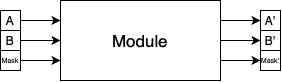
\includegraphics[width=.5\textwidth]{figures/Module.png}
  \caption{A Module, the main building block of a pipeline.}
\end{figure}

Since the pipelines are composed of mostly independent modules that operate on two input images and in some cases its mask, a flexible framework has been designed to model this behaviour. A \textit{pipeline} contains a sequence of modules that by default are fed the output of the preceding one. This behavior can be modified to suit the pipeline's needs by specifying the id of the module whose output will be chosen as input. Pipelines themselves can be used as modules to organize the code better. A small example of the syntax used for the registration section of the Fourier-Mellin Pipeline is shown below:

\begin{lstlisting}[
    caption={Example of pipeline definition},
    label=lst:pipeline-definition,
    language=Python]
registration_id, registration = Pipeline('registration')
start_id, _ = registration.add_module(IdentityModule())
registration.add_module(FourierModule())
registration.add_module(LogPolarModule(order=1))
registration.add_module(PhaseCorrelationModule(10, 'rotation'))
registration.add_module(IdentityModule(), input_stage=start_id)
registration.add_module(WarpModule(), apply_to=('b', 'm'))
registration.add_module(PhaseCorrelationModule(10, 'translation'))
\end{lstlisting}

The \lstinline{add_module} method on the pipeline allows us to specify a module, the input stage, and to which of the inputs apply the functionality. The reroute-able inputs work by caching the output of each module in the pipeline itself. If rerouting is specified, the pipeline will use these cached values instead of using the output of the previous module. In addition the pipeline itself, on initialization, can take arguments to aid in debugging by printing the output of the pipeline at that stage. It is the hope that this will make it easier to iterate on or modify the code by swapping out modules or extending pipelines. All this functionality however, comes with the additional cost in memory to hold the cached values of the pipeline during the cycle. A fully optimized, monolithic pipeline would be more efficient and might be the right step when working towards implementing this in the \acrshort{rov}, however this approach offers the flexibility needed during this experimentation phase.

In most cases the modules perform the same operations on the inputs, in which case it would be advantageous to perform these tasks in parallel. To simplify the implementation of parallelization, the modules use \texttt{Ray} from Anyscale, Inc. Processing only on the CPU is not the most efficient, but by parallelizing the pipeline where possible some speedup can be gained.

Parallelization using \texttt{Ray} is done using \texttt{Tasks}. These turn static methods into asynchronously executable functions, ideally helping us to halve the time it takes to execute a module. In essence, any static function is a candidate for this. Note the \lstinline{@ray.remote} in the following example of a module using \texttt{Ray}:

\begin{lstlisting}[
    caption={Example of pipeline parallelization},
    label=lst:pipeline-parallelization,
    language=Python]
class BandpassModule(PipelineModule):
    def __init__(self, low_cutoff, high_cutoff):
        super().__init__()
        self.low_cutoff = low_cutoff
        self.high_cutoff = high_cutoff

    @staticmethod
    @ray.remote
    def bandpass(data, low_cutoff, high_cutoff):
        if data is None:
            return None
        return difference_of_gaussians(data, low_cutoff, high_cutoff)

    def run(self, a, b, mask, tform, error):
        a = self.bandpass.remote(a, self.low_cutoff, self.high_cutoff)
        b = self.bandpass.remote(b, self.low_cutoff, self.high_cutoff)
        return ray.get(a), ray.get(b), mask, tform, error
\end{lstlisting}

\section{\citeauthor{Reddy1996}'s Fourier-Mellin Pipeline (adapted) \cite{Reddy1996}}
\label{sec:fmpipeline}
\begin{figure}[H] 
  \centering
  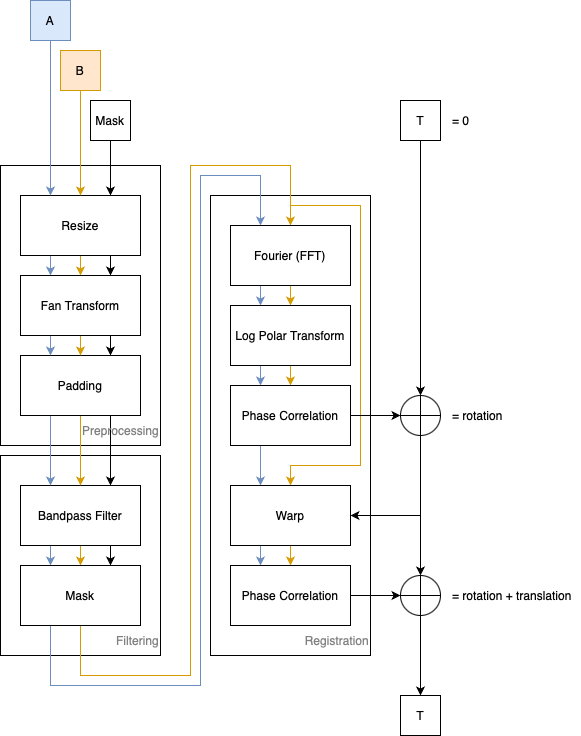
\includegraphics[width=.7\textwidth]{figures/fourier_mellin_pipeline.png}
  \caption{Block diagram of the Fourier-Mellin registration pipeline (adapted).}
  \label{fig:fmpipeline}
\end{figure}

The Fourier-Mellin Pipeline has been adapted to suit sonar images in a total of 10 independent modules. The main adaptation is the addition of the first block of modules (Resizing, Fan Transformation and Padding) which allows the Fourier-Mellin Pipeline to work on sonar images. Note that most of them are fed their inputs sequentially, except for the Warp Module which applies the detected rotation to the masked image so that the translation could be identified. Here, the flexibility of the pipeline framework implementation shines. The next sections will go into more detail about how each module is implemented. 

\begin{lstlisting}[
    caption={Fourier-Mellin Pipeline Implementation},
    label=lst:fm-pipeline-code,
    language=Python]
pipeline = Pipeline(output=args.out, 
                    intermediate_output=args.intermediate_output, 
                    verbose=args.verbose)
pipeline.add_module(IdentityModule())
conditioning_id, conditioning = pipeline.add_module(Pipeline('conditioning'))
conditioning.add_module(ResizeModule(args.resize))
conditioning.add_module(FanModule(bearings, output=args.out))
conditioning.add_module(PaddingModule(0.25))

pipeline.add_module(MetricsModule(output=args.out))

filtering_id, filtering = pipeline.add_module(Pipeline('filtering'))
filtering.add_module(BandpassModule(args.bandpass_low, args.bandpass_high))
filtering.add_module(MaskModule(padding=60, sigma=15))

registration_id, registration = pipeline.add_module(Pipeline('registration'))
start_id, _ = registration.add_module(IdentityModule())
registration.add_module(FourierModule())
registration.add_module(LogPolarModule(order=1))
registration.add_module(PhaseCorrelationModule(10, 'rotation'))
registration.add_module(IdentityModule(), input_stage=start_id)
registration.add_module(WarpModule(), apply_to=('b', 'm'))
registration.add_module(PhaseCorrelationModule(10, 'translation'))

pipeline.add_module(UpdateTformModule(range_resolution=range_resolution))
pipeline.add_module(IdentityModule(), ('a', 'b'), input_stage=conditioning_id)
pipeline.add_module(WarpModule(combine=True), 'b')
pipeline.add_module(OdometerModule(output=args.out, 
                                   range_resolution=range_resolution))
\end{lstlisting}

\section{\citeauthor{Hurtos2015} Pipeline \cite{Hurtos2015}}
\begin{figure}[H] 
  \centering
  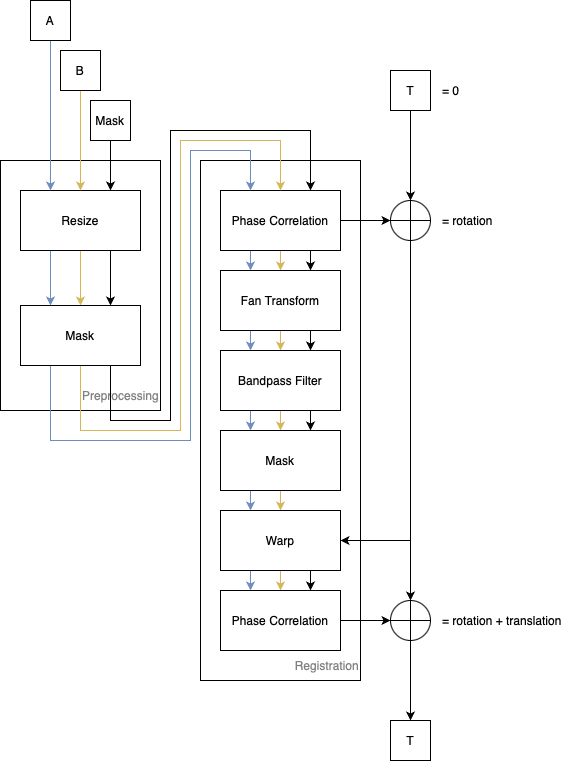
\includegraphics[width=.7\textwidth]{figures/reddy_pipeline.png}
  \caption{Block diagram of \citeauthor{Hurtos2015}'s Pipeline (adapted).}
  \label{fig:pcpipeline}
\end{figure}

With 9 modules \citeauthor{Hurtos2015}'s Pipeline isn't much shorter on first inspection. On a closer look however, it is evident that some of the heavyweight modules from the Fourier-Mellin pipeline are missing: Fourier Transform and the Log-Polar transform. As mentioned before, performing Phase Correlation over the raw polar image although faster and valid for short rotations, might not perform so well on distant frames. This is because the rotations isn't decoupled from translations in the raw sonar frame. Given the frequency of sonar frames coming from the \acrshort{bsosonar} (see \autoref{tab:sonar_specs}) and the max speed of the drone (see \autoref{tab:drone_specs}, we can assume that translations will be very small. At \(10Hz\) there is \(0.1s\) between frames. At \(1.5m/s\) the maximum movement between frames would be \(0.15m\). This is a small value indeed, but gets even smaller when considering that the drone is observing the seabed at significant distance. 

\begin{lstlisting}[
    caption={\citeauthor{Hurtos2015} Pipeline Implementation},
    label=lst:pc-pipeline-code,
    language=Python]
pipeline = Pipeline(output=args.out, 
                    intermediate_output=args.intermediate_output, 
                    verbose=args.verbose)
registration_id, registration = pipeline.add_module(Pipeline('registration'))
registration.add_module(ResizeModule(args.resize))
resize_id, _ = registration.add_module(IdentityModule())
registration.add_module(MaskModule(padding=60, sigma=15))
registration.add_module(PhaseCorrelationModule(20, 'rotation', log_polar=False))
registration.add_module(FanModule(bearings, output=args.out), input_stage=resize_id)
padding_id, _ = registration.add_module(PaddingModule(0.25))
registration.add_module(BandpassModule(args.bandpass_low, args.bandpass_high))
registration.add_module(MaskModule(padding=60, sigma=15))
registration.add_module(WarpModule(), apply_to=('b', 'm'))
registration.add_module(PhaseCorrelationModule(10, 'translation'))
pipeline.add_module(UpdateTformModule())
pipeline.add_module(IdentityModule(), ('a', 'b'), input_stage=pipeline.name)
pipeline.add_module(OdometerModule(output=args.out, 
                                   range_resolution=range_resolution))
pipeline.add_module(IdentityModule(), input_stage=padding_id)
pipeline.add_module(WarpModule(combine=True), 'b')
\end{lstlisting}



\section{Pre-processing pipelines' modules}

Many modules are used in both pipelines and are worth mentioning here.
\begin{itemize}
    \item Resizing: mainly down-sampling, is essential for speeding up the processing pipeline as it reduces the computations needed down the line. Often the starting point of the pipeline. Taking as input a resizing ratio \(R\) it calculates the expected size of the resized image and re-scales it appropriately. Down-sampling with an anti-aliasing filter also also reduces noise, another positive side-effect of this module.
    \item Padding: necessary for keeping the sonar image in frame once the rotation is applied. A black border is added to the image to keep the relevant data in frame.
    \item Filtering: it is recommended to apply some degree of band-pass filtering focusing in particular on high frequency noise.
    \item Masking: the images should be windowed to have smooth borders to avoid spectral leakage from the image borders. This module applies some gaussian filtering to the current mask and applies it to the input images. This makes the image have a smoother transition from the border to the data.
\end{itemize}


\subsection{Resizing (down-sampling)}

\begin{figure}[H]
    \centering
    \begin{subfigure}[b]{.45\textwidth}
        \centering
        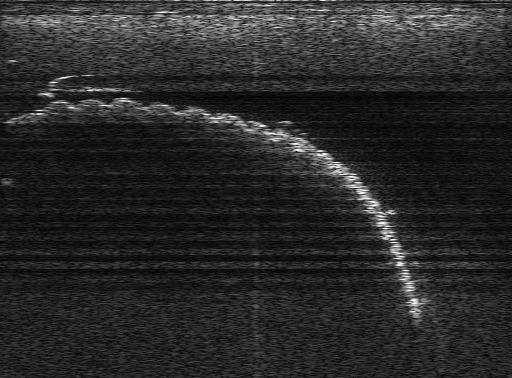
\includegraphics[width=\textwidth]{figures/pipeline/Original.png}
        \caption{Raw data obtained from the sonar}
    \end{subfigure}
    \hfill
    \begin{subfigure}[b]{.45\textwidth}
        \centering
        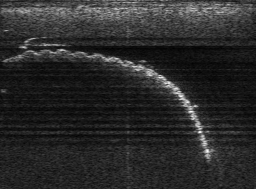
\includegraphics[width=\textwidth]{figures/pipeline/Resized.png}
        \caption{Resized frame}
    \end{subfigure}
    \caption{Down-sampled image}
    \label{fig:resizing}
\end{figure}

Resizing the images is necessary to make the pipelines in consideration less computationally expensive. This is a "low hanging fruit" optimization that yields visible results. This module takes images of size \((w, h)\) and re-scales them to \((w^*, h^*)\), given a resizing ratio \(R\) where:

\[w^* = w\sqrt{R}\]
\[h^* = h\sqrt{R}\]

In code this is achieved using the \texttt{skimage.transform.resize} package using:

\begin{lstlisting}[
    caption={Resizing code},
    label=lst:pipeline-resizing,
    language=Python]
ratio = np.sqrt(R)
img = resize(img.copy(), 
             (int(img.shape[0] * ratio), int(img.shape[1] * ratio)), 
             anti_aliasing=True)
\end{lstlisting}

The \lstinline{anti_aliasing=True} is necessary to avoid the introduction of aliasing artifacts through down-sampling. Down-sampling an image has the secondary function of acting as a kind of averaging filter which will also work towards reducing the noise in the image. 

Later on, in the results section, the speedup resulting from down-sampling of the image will be evaluated. It is also important to mention that since operations are done independently on each input image, this is a perfect candidate for parallelization over its inputs with \texttt{Ray}.

\subsection{Padding}

\begin{figure}[H]
    \centering
    \begin{subfigure}[b]{.45\textwidth}
        \centering
        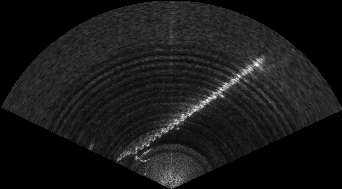
\includegraphics[width=\textwidth]{figures/pipeline/Fan.png}
        \caption{Input fan frame}
    \end{subfigure}
    \hfill
    \begin{subfigure}[b]{.45\textwidth}
        \centering
        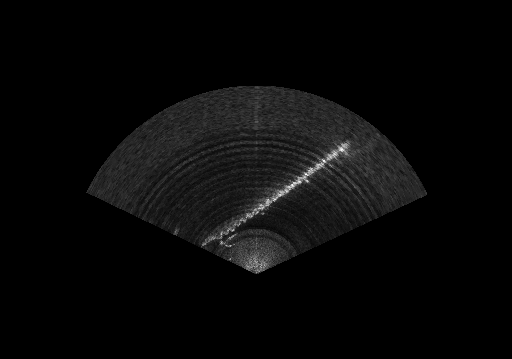
\includegraphics[width=\textwidth]{figures/pipeline/Padding.png}
        \caption{Padded fan frame}
    \end{subfigure}
    \caption{Padded image}
    \label{fig:resizing}
\end{figure}

Especially necessary for images that have undergone their Fan Transformation and will be rotated. Any rotation applied to the image might make some of its data go beyond the edges. Adding some padding ensures that all the sonar data remains inside the image. The module takes in a padding ratio \(r\) and pads the image with a black border with a width of \(r * max(widht, height)\). By default, the padding ratio is chosen to be \texttt{0.25}. Smaller values could be chosen, but this may affect registration of distant frames. Choosing this parameter depends on two things: how distant the frames are (big rotations and translations) and the computational impact of more pixels downstream in the pipeline.

In code this is implemented using numpy as:
\begin{lstlisting}[
    caption={Padding code},
    label=lst:pipeline-padding,
    language=Python]
pad_size = int(np.max(img.shape) * self.padding_ratio)
np.pad(data, pad_size, mode='constant', constant_values=0)
\end{lstlisting}

Again, since there are no dependecies between the images, this is a perfect candidate for parallelization using \texttt{Ray}.

\section{Filtering}

\begin{figure}[H]
    \centering
    \begin{subfigure}[b]{.45\textwidth}
        \centering
        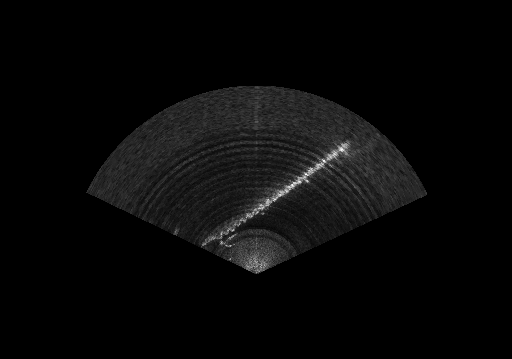
\includegraphics[width=\textwidth]{figures/pipeline/Padding.png}
        \caption{Input padded fan frame}
    \end{subfigure}
    \hfill
    \begin{subfigure}[b]{.45\textwidth}
        \centering
        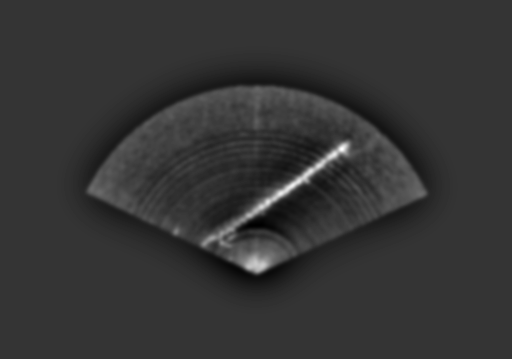
\includegraphics[width=\textwidth]{figures/pipeline/Bandpass.png}
        \caption{Band-passed padded fan frame}
    \end{subfigure}
    \caption{Band-passed image}
    \label{fig:resizing}
\end{figure}

If required by the pipeline, a band-pass filter has been implemented using \acrfull{dog}. This is a spatial-domain band-pass filter that also works as a feature enhancement algorithm. The filter generates two blurred versions of the original using Gaussian blur, where one of the images is more blurred than the other. The output results from subtracting the more blurry image from the less blurry one. It can enhance edges and other details present in the image while attenuating the noise, making it perfect for image registration.

The \acrshort{dog} takes two parameters \(\sigma_{low}\) and \(\sigma_{high}\). Choosing these values was done qualitatively to include some blurring and maximize contrast with features in the image.

\begin{figure}[H]
    \centering
    \begin{subfigure}[b]{.32\textwidth}
        \centering
        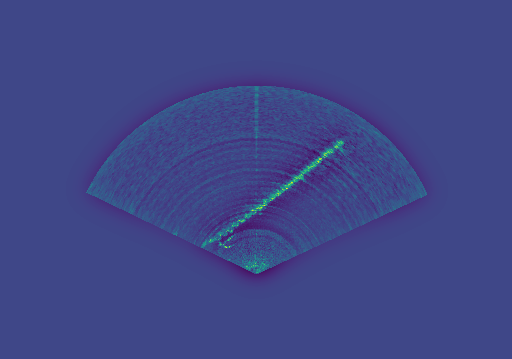
\includegraphics[width=\textwidth]{figures/bandpassing/0_10.png}
        \caption{\(\sigma_{low} = 0\) \(\sigma_{high} = 10\)}
    \end{subfigure}
    \hfill
    \begin{subfigure}[b]{.32\textwidth}
        \centering
        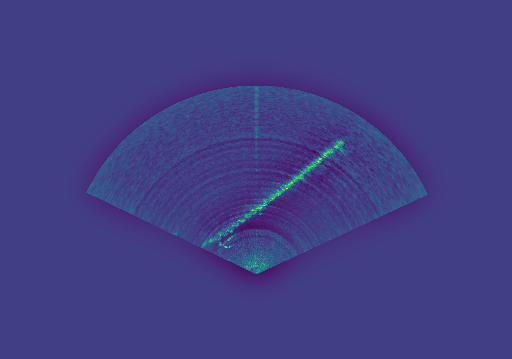
\includegraphics[width=\textwidth]{figures/bandpassing/0_15.png}
        \caption{\(\sigma_{low} = 0\) \(\sigma_{high} = 15\)}
    \end{subfigure}
    \hfill
    \begin{subfigure}[b]{.32\textwidth}
        \centering
        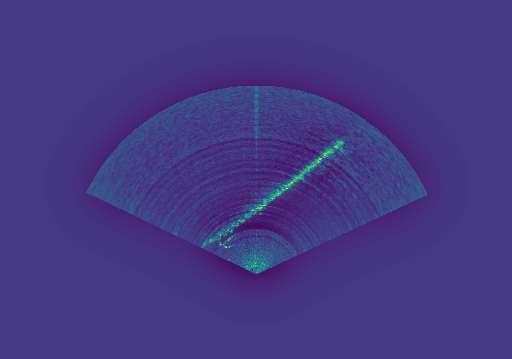
\includegraphics[width=\textwidth]{figures/bandpassing/0_20.png}
        \caption{\(\sigma_{low} = 0\) \(\sigma_{high} = 20\)}
    \end{subfigure}
    \hfill
    \begin{subfigure}[b]{.32\textwidth}
        \centering
        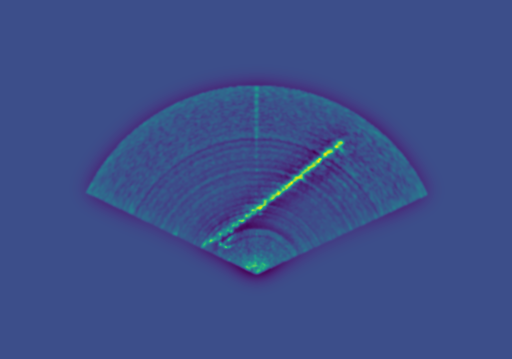
\includegraphics[width=\textwidth]{figures/bandpassing/1_10.png}
        \caption{\(\sigma_{low} = 1\) \(\sigma_{high} = 10\)}
    \end{subfigure}
    \hfill
    \begin{subfigure}[b]{.32\textwidth}
        \centering
        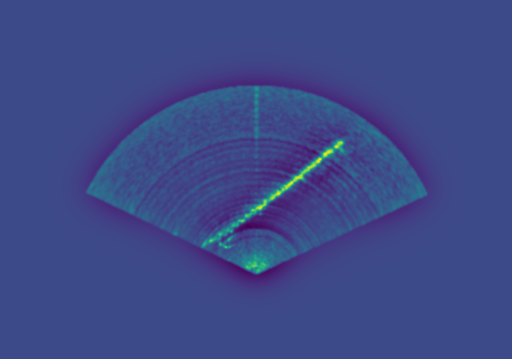
\includegraphics[width=\textwidth]{figures/bandpassing/1_15.png}
        \caption{\(\sigma_{low} = 1\) \(\sigma_{high} = 15\)}
    \end{subfigure}
    \hfill
    \begin{subfigure}[b]{.32\textwidth}
        \centering
        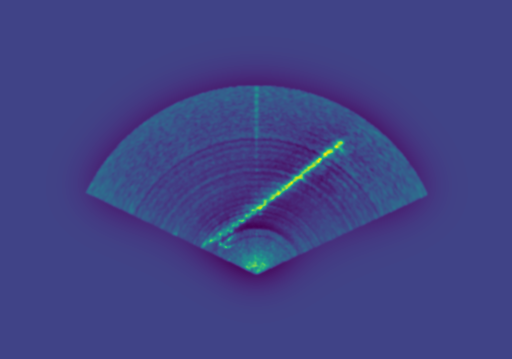
\includegraphics[width=\textwidth]{figures/bandpassing/1_20.png}
        \caption{\(\sigma_{low} = 1\) \(\sigma_{high} = 20\)}
    \end{subfigure}
    \hfill
    \begin{subfigure}[b]{.32\textwidth}
        \centering
        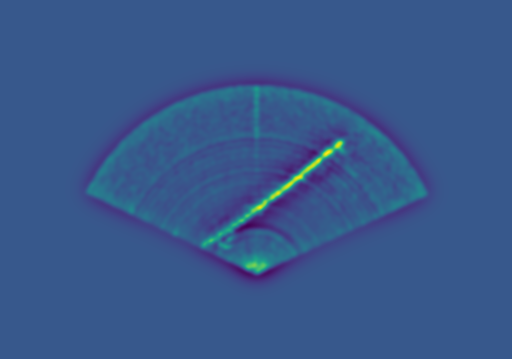
\includegraphics[width=\textwidth]{figures/bandpassing/2_10.png}
        \caption{\(\sigma_{low} = 2\) \(\sigma_{high} = 10\)}
    \end{subfigure}
    \hfill
    \begin{subfigure}[b]{.32\textwidth}
        \centering
        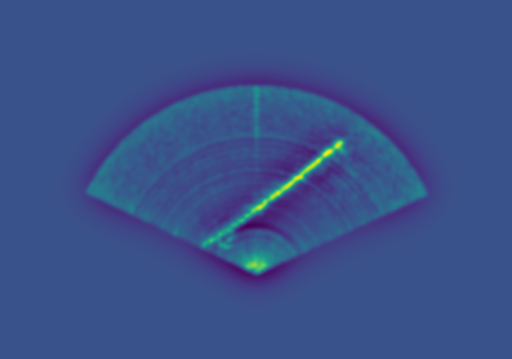
\includegraphics[width=\textwidth]{figures/bandpassing/2_15.png}
        \caption{\(\sigma_{low} = 2\) \(\sigma_{high} = 15\)}
    \end{subfigure}
    \hfill
    \begin{subfigure}[b]{.32\textwidth}
        \centering
        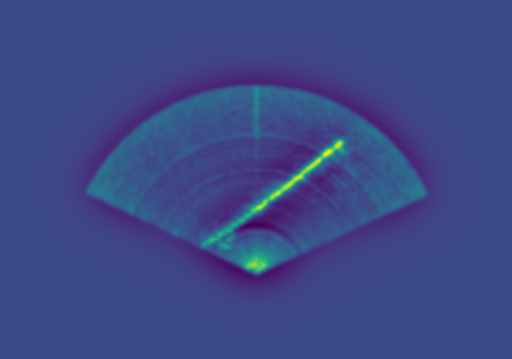
\includegraphics[width=\textwidth]{figures/bandpassing/2_20.png}
        \caption{\(\sigma_{low} = 2\) \(\sigma_{high} = 20\)}
    \end{subfigure}
    \hfill
    \begin{subfigure}[b]{.32\textwidth}
        \centering
        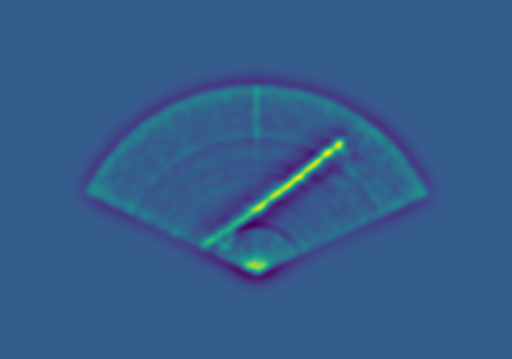
\includegraphics[width=\textwidth]{figures/bandpassing/3_10.png}
        \caption{\(\sigma_{low} = 3\) \(\sigma_{high} = 10\)}
    \end{subfigure}
    \hfill
    \begin{subfigure}[b]{.32\textwidth}
        \centering
        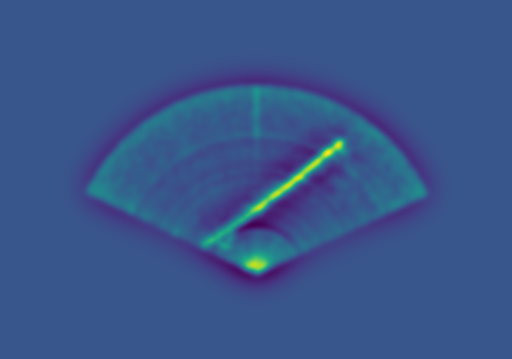
\includegraphics[width=\textwidth]{figures/bandpassing/3_15.png}
        \caption{\(\sigma_{low} = 3\) \(\sigma_{high} = 15\)}
    \end{subfigure}
    \hfill
    \begin{subfigure}[b]{.32\textwidth}
        \centering
        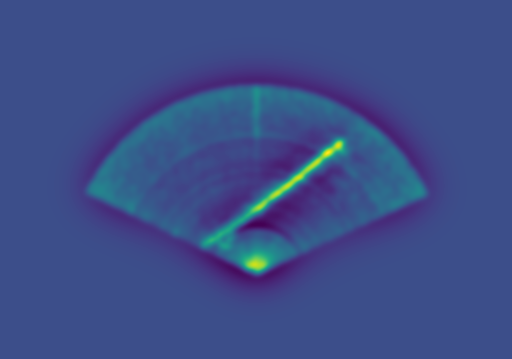
\includegraphics[width=\textwidth]{figures/bandpassing/3_20.png}
        \caption{\(\sigma_{low} = 3\) \(\sigma_{high} = 20\)}
    \end{subfigure}
    \caption{Choosing \(\sigma_{low}\) and \(\sigma_{high}\) values for band-passing}
    \label{fig:resizing}
\end{figure}

Combination \(\sigma_{low} = 2\) \(\sigma_{high} = 20\) is chosen as it accentuates contrast between empty background and features without losing too much detail in the blurring. It's very hard to justify why these parameters would best quantitatively. The metric to go to in this case would be \acrfull{snr}. However this is impossible to calculate without having a reference "true" signal. These parameters can be changed easily from the \acrshort{cli} if desired. In code this filter is implemented through the \texttt{skimage.filters.difference\_of\_gaussians} package:

\begin{lstlisting}[
    caption={Bandpassing code},
    label=lst:pipeline-bandpassing,
    language=Python]
difference_of_gaussians(img, low_sigma, high_sigma)
\end{lstlisting}

Once more, this is a perfect candidate for parallelization using \texttt{Ray}.

\subsection{Masking}

As mentioned before, when applying a discrete Fourier transform if the input isn't periodic this might result in "spectral leakage". This shows up as random frequencies that aren't really part of the input. To avoid this, some windowing of the image is required. As part of the inputs of the pipeline a mask is provided which might be transformed by some of the modules. For example the Fan Transformation Module will convert the rectangular input mask into the fan shape. By default the input mask to the pipeline is an array of ones with the same shape as a sonar frame. The masking module takes the input mask, reduces the size of the masking area while preserving the image size, and applies some gaussian filtering to it with the purpose of smoothing its edges:

\begin{figure}[H]
    \centering
    \begin{subfigure}[b]{.45\textwidth}
        \centering
        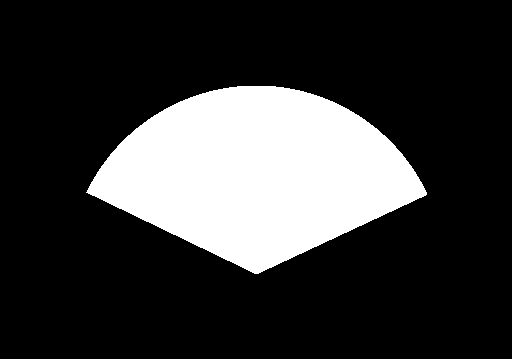
\includegraphics[width=\textwidth]{figures/pipeline/Mask.png}
        \caption{Fan mask}
    \end{subfigure}
    \hfill
    \begin{subfigure}[b]{.45\textwidth}
        \centering
        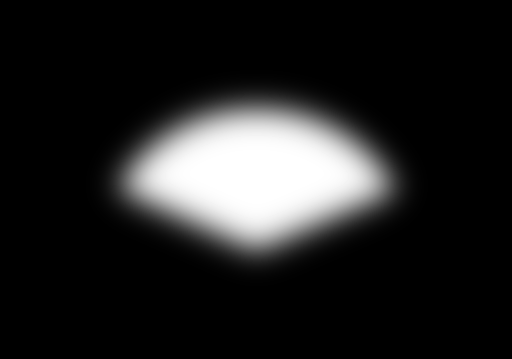
\includegraphics[width=\textwidth]{figures/pipeline/MaskBlurred.png}
        \caption{Smoothed \& resized mask}
    \end{subfigure}
    \caption{Smoothing the mask}
    \label{fig:mask-smoothing}
\end{figure}

A padding of \texttt{60px} on every side was chosen as after resizing back to the orignal image size, it makes the blurred border fit completely inside the original mask. In code this is implemented using \texttt{numpy}, \texttt{scipy.ndimage.gaussian\_filter} and \texttt{skimage.transform.resize}:

\begin{lstlisting}[
    caption={Smoothed mask code},
    label=lst:pipeline-masking-smoothing,
    language=Python]
# Add black border
padding = 60
mask = np.pad(input_mask, padding, mode='constant', constant_values=0)
# Resize mask to orignal size
mask = resize(mask, input_mask.shape, anti_aliasing=True)
# Gaussian blur the mask
mask = gaussian_filter(mask, sigma=self.sigma)
\end{lstlisting}

Another optimization takes place here. Instead of recalculating this mask for every incoming frame, the mask is cached and reused in the future. The caching implementation is very simple so the restriction of all frames being the same size still applies. This mask is then applied to the input frames to reduce the visibility of the border of the sonar frame:

\begin{figure}[H]
    \centering
    \begin{subfigure}[b]{.45\textwidth}
        \centering
        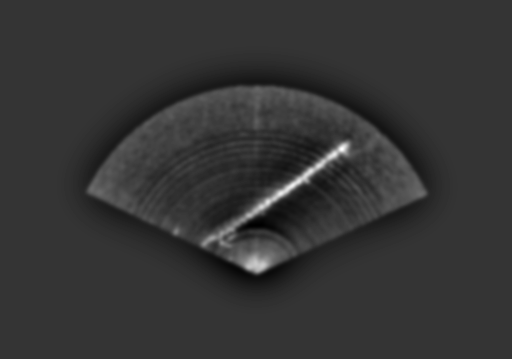
\includegraphics[width=\textwidth]{figures/pipeline/Bandpass.png}
        \caption{Unmasked frame}
    \end{subfigure}
    \hfill
    \begin{subfigure}[b]{.45\textwidth}
        \centering
        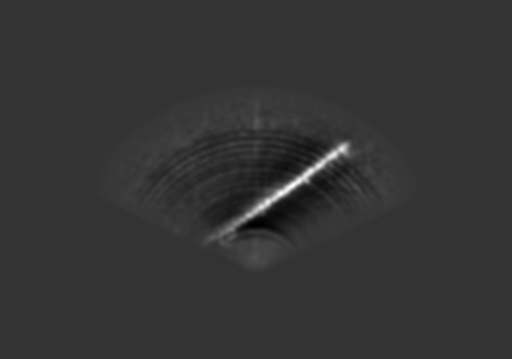
\includegraphics[width=\textwidth]{figures/pipeline/Masking.png}
        \caption{Masked frame}
    \end{subfigure}
    \caption{Applying the mask}
    \label{fig:mask-smoothing}
\end{figure}

Using \texttt{numpy} this can be easily achieved through element-wise multiplication: \lstinline{image * mask}. Yet again, except for the calculation of the mask the first time the module runs, this is a perfect candidate for parallelization using \texttt{Ray}.

\section{Fan Transformation}
One of the main modules is definitely the Fan Transformation Module. The raw data from the sensor is structured in an array that represents ping intensity at a specific bearing and range. It is important to note that the beam bearings are not evenly spaced. The sensor provides a table that accompanies the ping information with the specific angle associated with each ping. All of this data is obtained through recording files stored on the \acrshort{rov}. These files contain the sonar data packed in a "Protocol Buffers" format specified by Blueye's Protocol Definitions \cite{Blueye:ProtocolDefinitions}. The following is an example "MultibeamPing" message:

\begin{lstlisting}[
    caption={Example MultibeamPing message},
    label=lst:ping-protobuf]
ping {
  range: 30.758804321289062
  gain: 100.0
  frequency: 1196808.5106382978
  speed_of_sound_used: 1517.4982581645493
  frequency_mode: MULTIBEAM_FREQUENCY_MODE_LOW_FREQUENCY
  number_of_ranges: 378
  number_of_beams: 512
  step: 512
  bearings: -65.0
  bearings: -64.5199966430664
  ...
  bearings: 64.5199966430664
  bearings: 65.0
  ping_data: [1D array containing sonar image]
  device_id: GUEST_PORT_DEVICE_ID_BLUEPRINT_SUBSEA_OCULUS_M1200D
}
\end{lstlisting}

The \lstinline{ping_data} is produced as a continuous 1D array that must be reshaped in order to work with it as an image. Using the \lstinline{number_of_ranges} and \lstinline{number_of_beams} we can convert the 1D-array into a 2D one. Using the equations from \ref{sec:fan-tform} and the bearing table provided by the MultibeamPing record, the fan transformation can be implemented as a module in the pipelines. 

A huge optimization can be performed here. Given the restriction that all the frames should have the same range and number of beams, the mapping can be pre-computed for all images and cached for use on all the incoming frames. This saves cpu cycles on performing all the possible \((u, v) \rightarrow (\theta,r)\) calculations. The effect of this speedup will be evaluated in the following sections.

Range resolution depends on the sonar, in our case 2.5mm per pixel along the range axis \ref{tab:sonar_specs}. It allows us to convert simple pixel values into real world coordinates. In most cases, a simple division of \lstinline{range} over \lstinline{number_of_ranges} will give us this value. However, it is often the case that to speed up processing images are resized. If the image is scaled a simple calculation can compensate for this change. Given \(R\) as the resizing ratio for the image area, the resizing ratio for a dimension of the image will be given by \(\sqrt{R}\). The new range resolution can be calculated with the following equation:

\[rangeResolution = \frac{range}{numberOfRanges * \sqrt{R}}\]

This module is yet another example of a candidate for parallelization using \texttt{Ray}.

\section{Registration Modules}



\subsection{\acrfull{fft}}

A simple module that applies the \acrshort{fft} to incoming inputs. The \acrshort{fft} is an algorithm that implements the Discrete Fourier Transform efficiently. The result of the transform is a signal in the complex domain (composed of Real and Imaginary parts). Decomposition into magnitude and phase makes it easier to visualize, and as mentioned previously in \autoref{sec:fm-registration} we're only interested in the magnitude for rotation estimation using \citeauthor{Reddy1996}'s Fourier-Mellin Pipeline. Using \texttt{numpy} we can get the magnitude of the \acrshort{fft} and center the zero-frequency component with: \lstinline{np.abs(np.fft.fftshift(np.fft.fft2(image)))}. This results in the following transformation:

\begin{figure}[H]
    \centering
    \begin{subfigure}[b]{.45\textwidth}
        \centering
        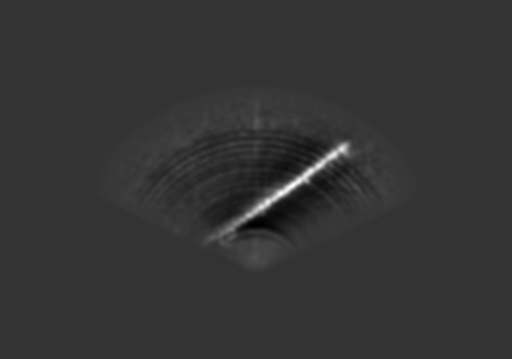
\includegraphics[width=\textwidth]{figures/pipeline/Masking.png}
        \caption{Masked frame}
    \end{subfigure}
    \hfill
    \begin{subfigure}[b]{.45\textwidth}
        \centering
        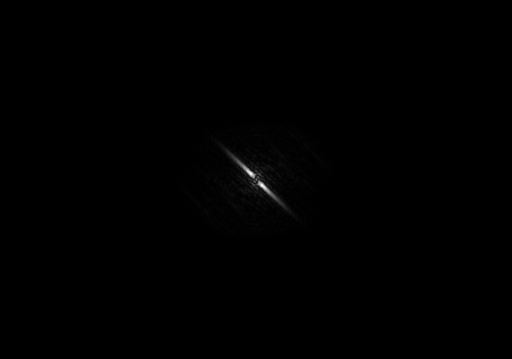
\includegraphics[width=\textwidth]{figures/pipeline/FFT.png}
        \caption{FFT}
    \end{subfigure}
    \caption{Fourier transform}
    \label{fig:fft}
\end{figure}


\subsection{Log-Polar Transform}

\subsection{Phase Correlation}

\section{Mosaicing}
\chapter{Experimental Setup}
\label{chap:setup}

This chapter will explain the experimental setup and how the experiments are set up for performance comparison.

To test the performance of the pipelines in an ideal setup and have a known reference to compare to, the experiments will be performed first using artificially generated data. Whenever generated sonar data is used, the frames come from the same source image that represents the seabed.

\begin{figure}[H]
  \centering
  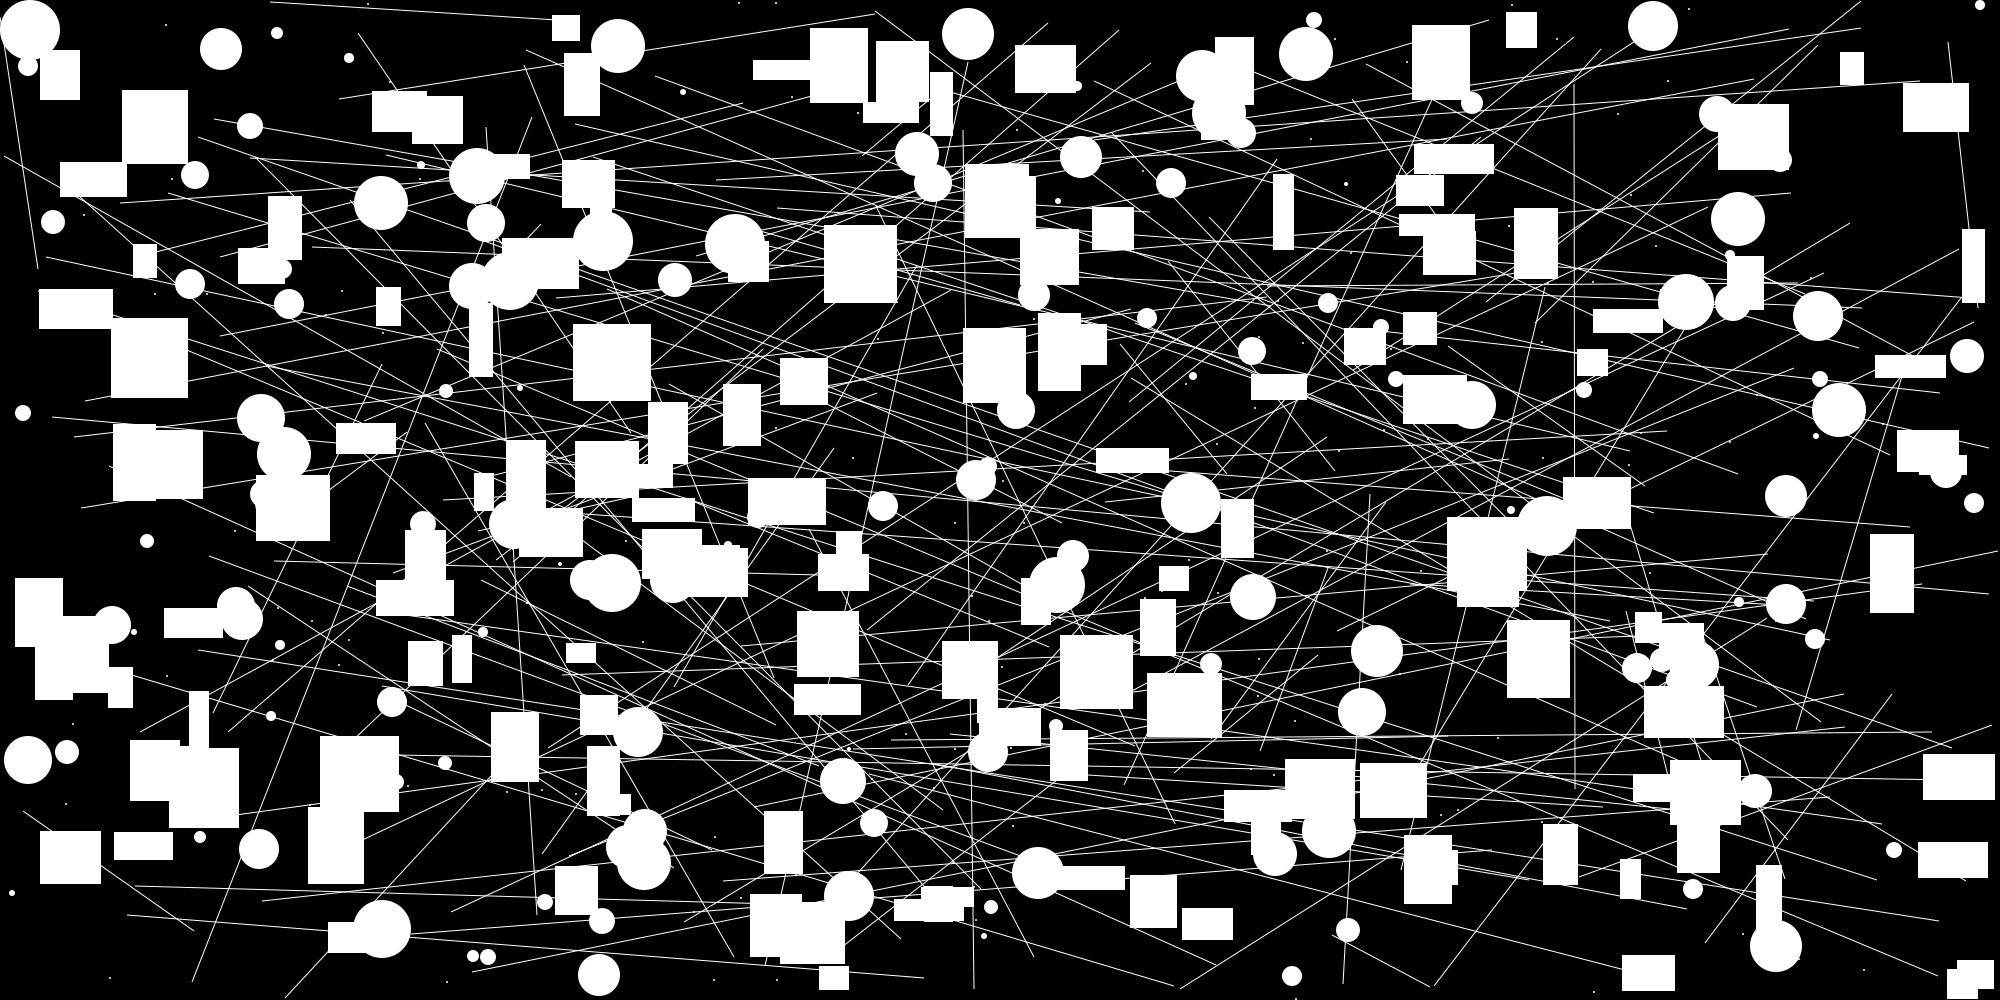
\includegraphics[width=.7\textwidth]{figures/setup/test-reference.png}
  \caption[Source image for fake data]{Artificially generated image used as reference for test sets}
  \label{fig:test_reference}
\end{figure}

For the sake of simplicity, one pixel in this image represents one meter. This will make evaluating the performance easier based on the measured translations.

Tests using real data use recordings from this area in Trondheim:
\begin{figure}[H]
  \centering
  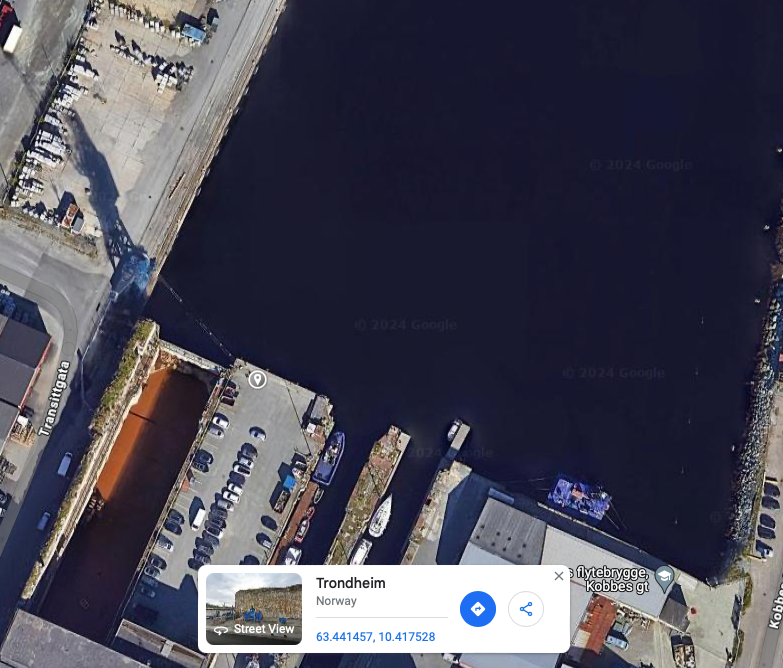
\includegraphics[width=.7\textwidth]{figures/setup/Map.png}
  \caption{Trondheim Harbor testing site: 63.441457, 10.417528}
  \label{fig:marina}
\end{figure}


To test rotation and translation, three sets of artificial data have been generated:

\begin{enumerate}
    \item Rotation: between each frame, there's a rotation of 1º.
    \item Translation (sway): performing a sideways translation of 10 px at every step, for a total displacement of 1000px.
    \item Translation (surge): performing a forward translation of 10 px at every step, for a total displacement of 1000px.
\end{enumerate}


As it is interesting to see how the pipelines estimate rotations and translations on distant frames, the test will be repeated skipping 0, 4, and 9 frames in between. This means that for rotations, an angular displacement of 1º, 5º, and 10º is expected on the estimation for each of the cases respectively. For translations, a horizontal displacement of 10 m, 50 m, and 100 m is expected.

Finally, the pipelines will be tested on real data captured through the \acrshort{rov}. Using the \acrshort{rov}'s DVL data as "ground truth", we can evaluate the accuracy of the measurements. The specs of the sonar used for these tests are the following:


\begin{table}[H]
    \centering
    \begin{tabular}{|c|c|}
        \hline
        \textbf{Parameter} & \textbf{Spec} \\ \hline
        Operating Frequency & 1.2 MHz / 2.1 MHz \\ \hline
        Range (Maximum) & 40 m / 10 m \\ \hline
        Range (Minimum) & 0.1 m \\ \hline
        Range Resolution & 2.5 mm / 2.5 mm \\ \hline
        Update Rate (Max.) & 40 Hz \\ \hline
        Horizontal Aperture & 130° / 60° \\ \hline
        Vertical Aperture & 20° / 12° \\ \hline
        Number of Beams (Max.) & 512 \\ \hline
        Angular Resolution & 0.6° / 0.4° \\ \hline
        Beam Separation & 0.25° / 0.16° \\ \hline
    \end{tabular}
    \caption{\acrlong{bsosonar} Specs \cite{BlueprintSubsea:Specs}.}
    \label{tab:sonar_specs}
\end{table}

The update rate was fixed through sonar settings to be 10Hz. The mentioned 40Hz can only be achieved on very small ranges. 

As mentioned before, the Blueye Robotics's X3 \acrshort{rov} will be used in this project. The drone can freely move along its sway, surge, and heave axes. However, for tests movement along the heave axis will be restricted so that the restrictions mentioned in \autoref{chap:implementation} apply. Using the DVL, the \acrshort{rov} can keep its altitude constant from the bottom. In addition, these are some of the drone's main specs:

\begin{table}[H]
    \centering
    \begin{tabular}{|c|c|}
        \hline
        \textbf{Parameter} & \textbf{Spec} \\ \hline
        Ingress protection & IPX8 \\ \hline
        Dimensions & 485 x 257 x 354 mm (LxWxH) \\ \hline
        Weight in air & 8.6 kg (with salt water ballast) \\ \hline
        Buoyancy material & HCP 30 Polymer Foam \\ \hline
        Maximum rated depth & 305 m \\ \hline
        Forward speed at normal use & 1.5 m/s (3 knots) \\ \hline
        Thrusters & 4 x 350 W \\ \hline
        Run time at normal use & 5 hours on High Capacity Battery \\ \hline
        Operating temperature & -10 to +50 °C \\ \hline
    \end{tabular}
    \caption{Blueye X3 \acrshort{rov} Specs \cite{Blueye:X3Specs}.}
    \label{tab:drone_specs}
\end{table}

All testing of software developed (the pipelines themselves) was performed on a MacBook Pro with an M1 Pro processor and 16GB of RAM.


\chapter{Results}
\label{chap:results}


\section{Rotation estimation}

% \begin{figure}[H] 
%   \centering
%   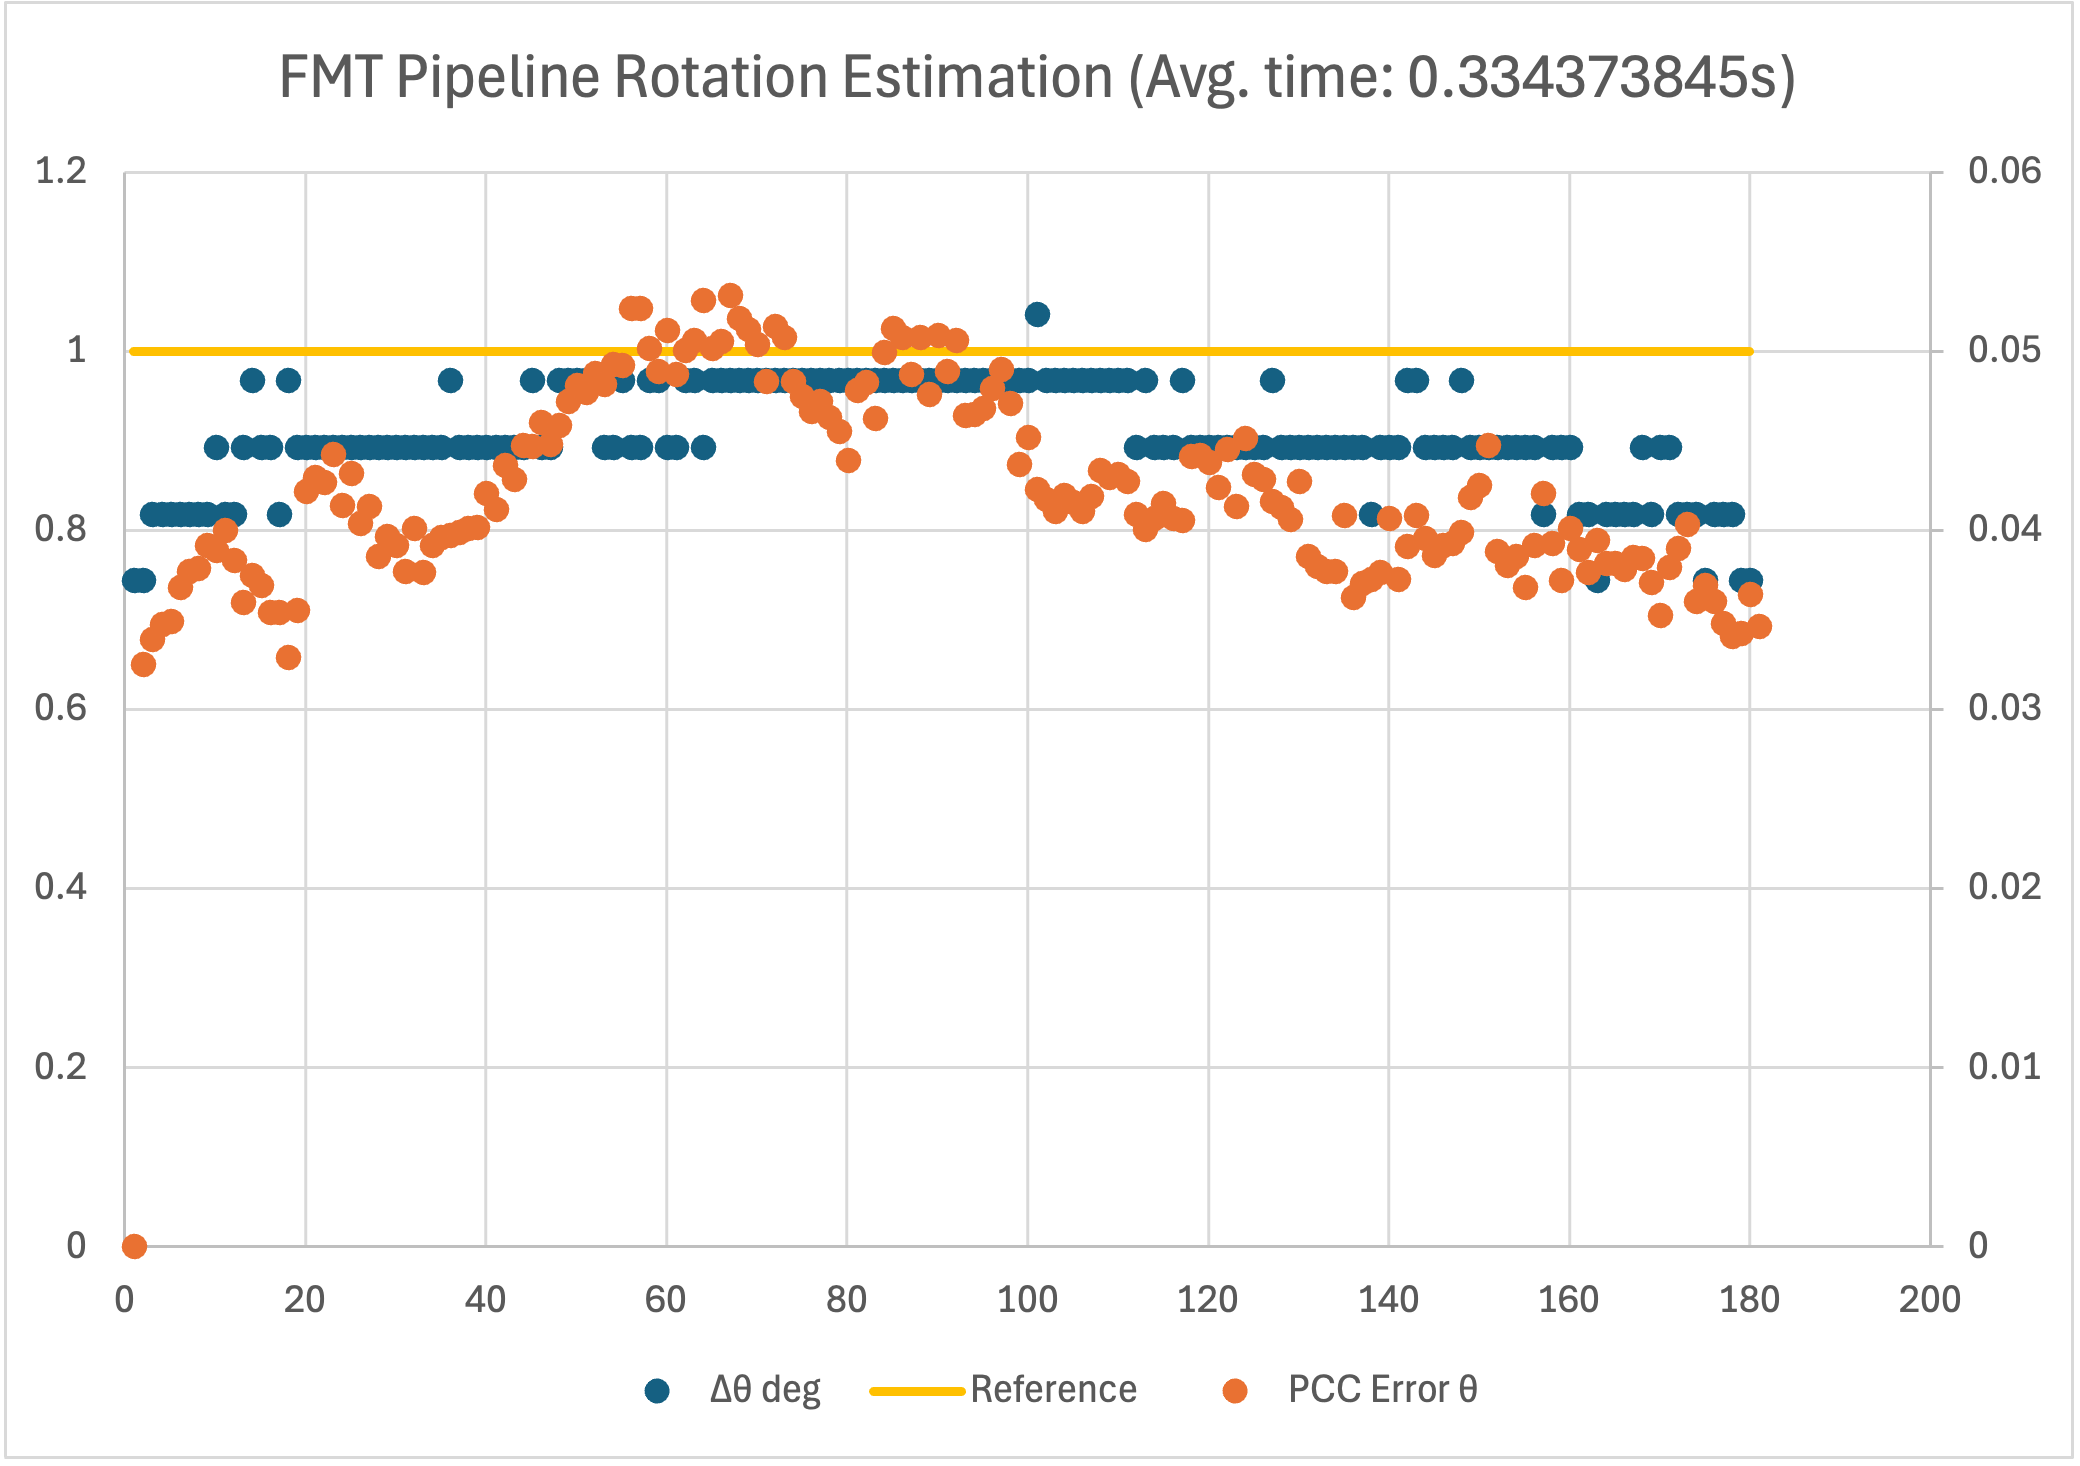
\includegraphics[width=.7\textwidth]{figures/results/rotation-skip-0/FMT-Rotation.png}
%   \caption[Fourier-Mellin Pipeline Rotation Estimation]{Rotation estimation using the Fourier-Mellin Pipeline}
%   \label{fig:fmrotation}
% \end{figure}


% \begin{figure}[H] 
%   \centering
%   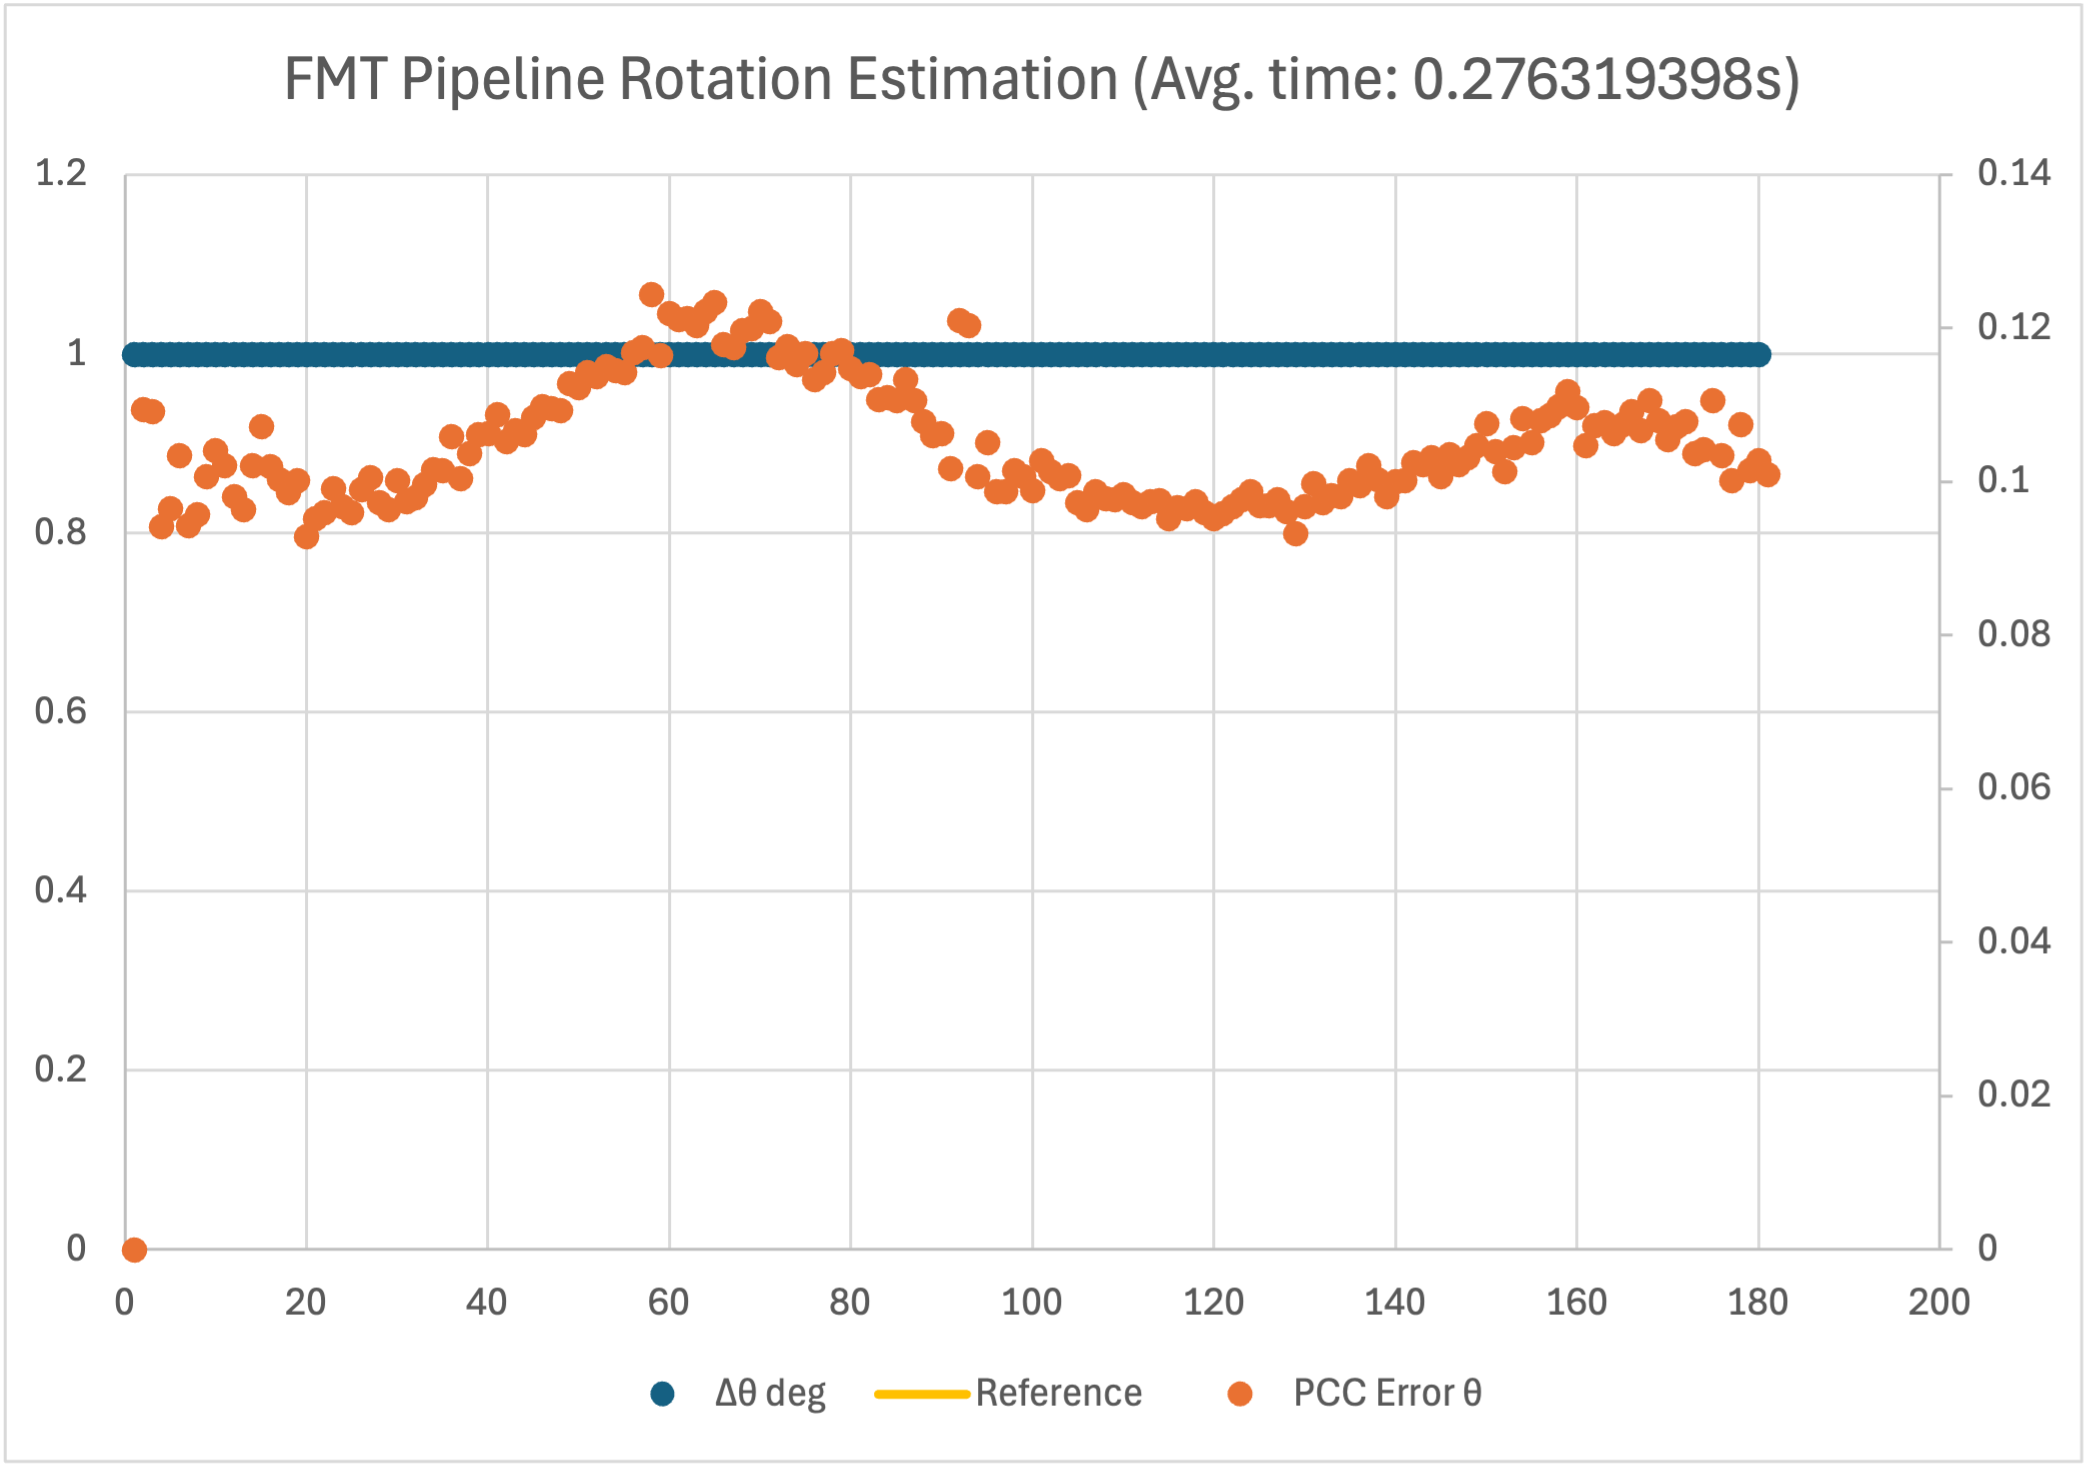
\includegraphics[width=.7\textwidth]{figures/results/rotation-skip-0/PC-Rotation.png}
%   \caption[\citeauthor{Hurtos2015} Pipeline Rotation Estimation]{Rotation estimation using the \citeauthor{Hurtos2015} Phase Correlation Pipeline}
%   \label{fig:pcrotation}
% \end{figure}
\begin{figure}[H]
  \centering
  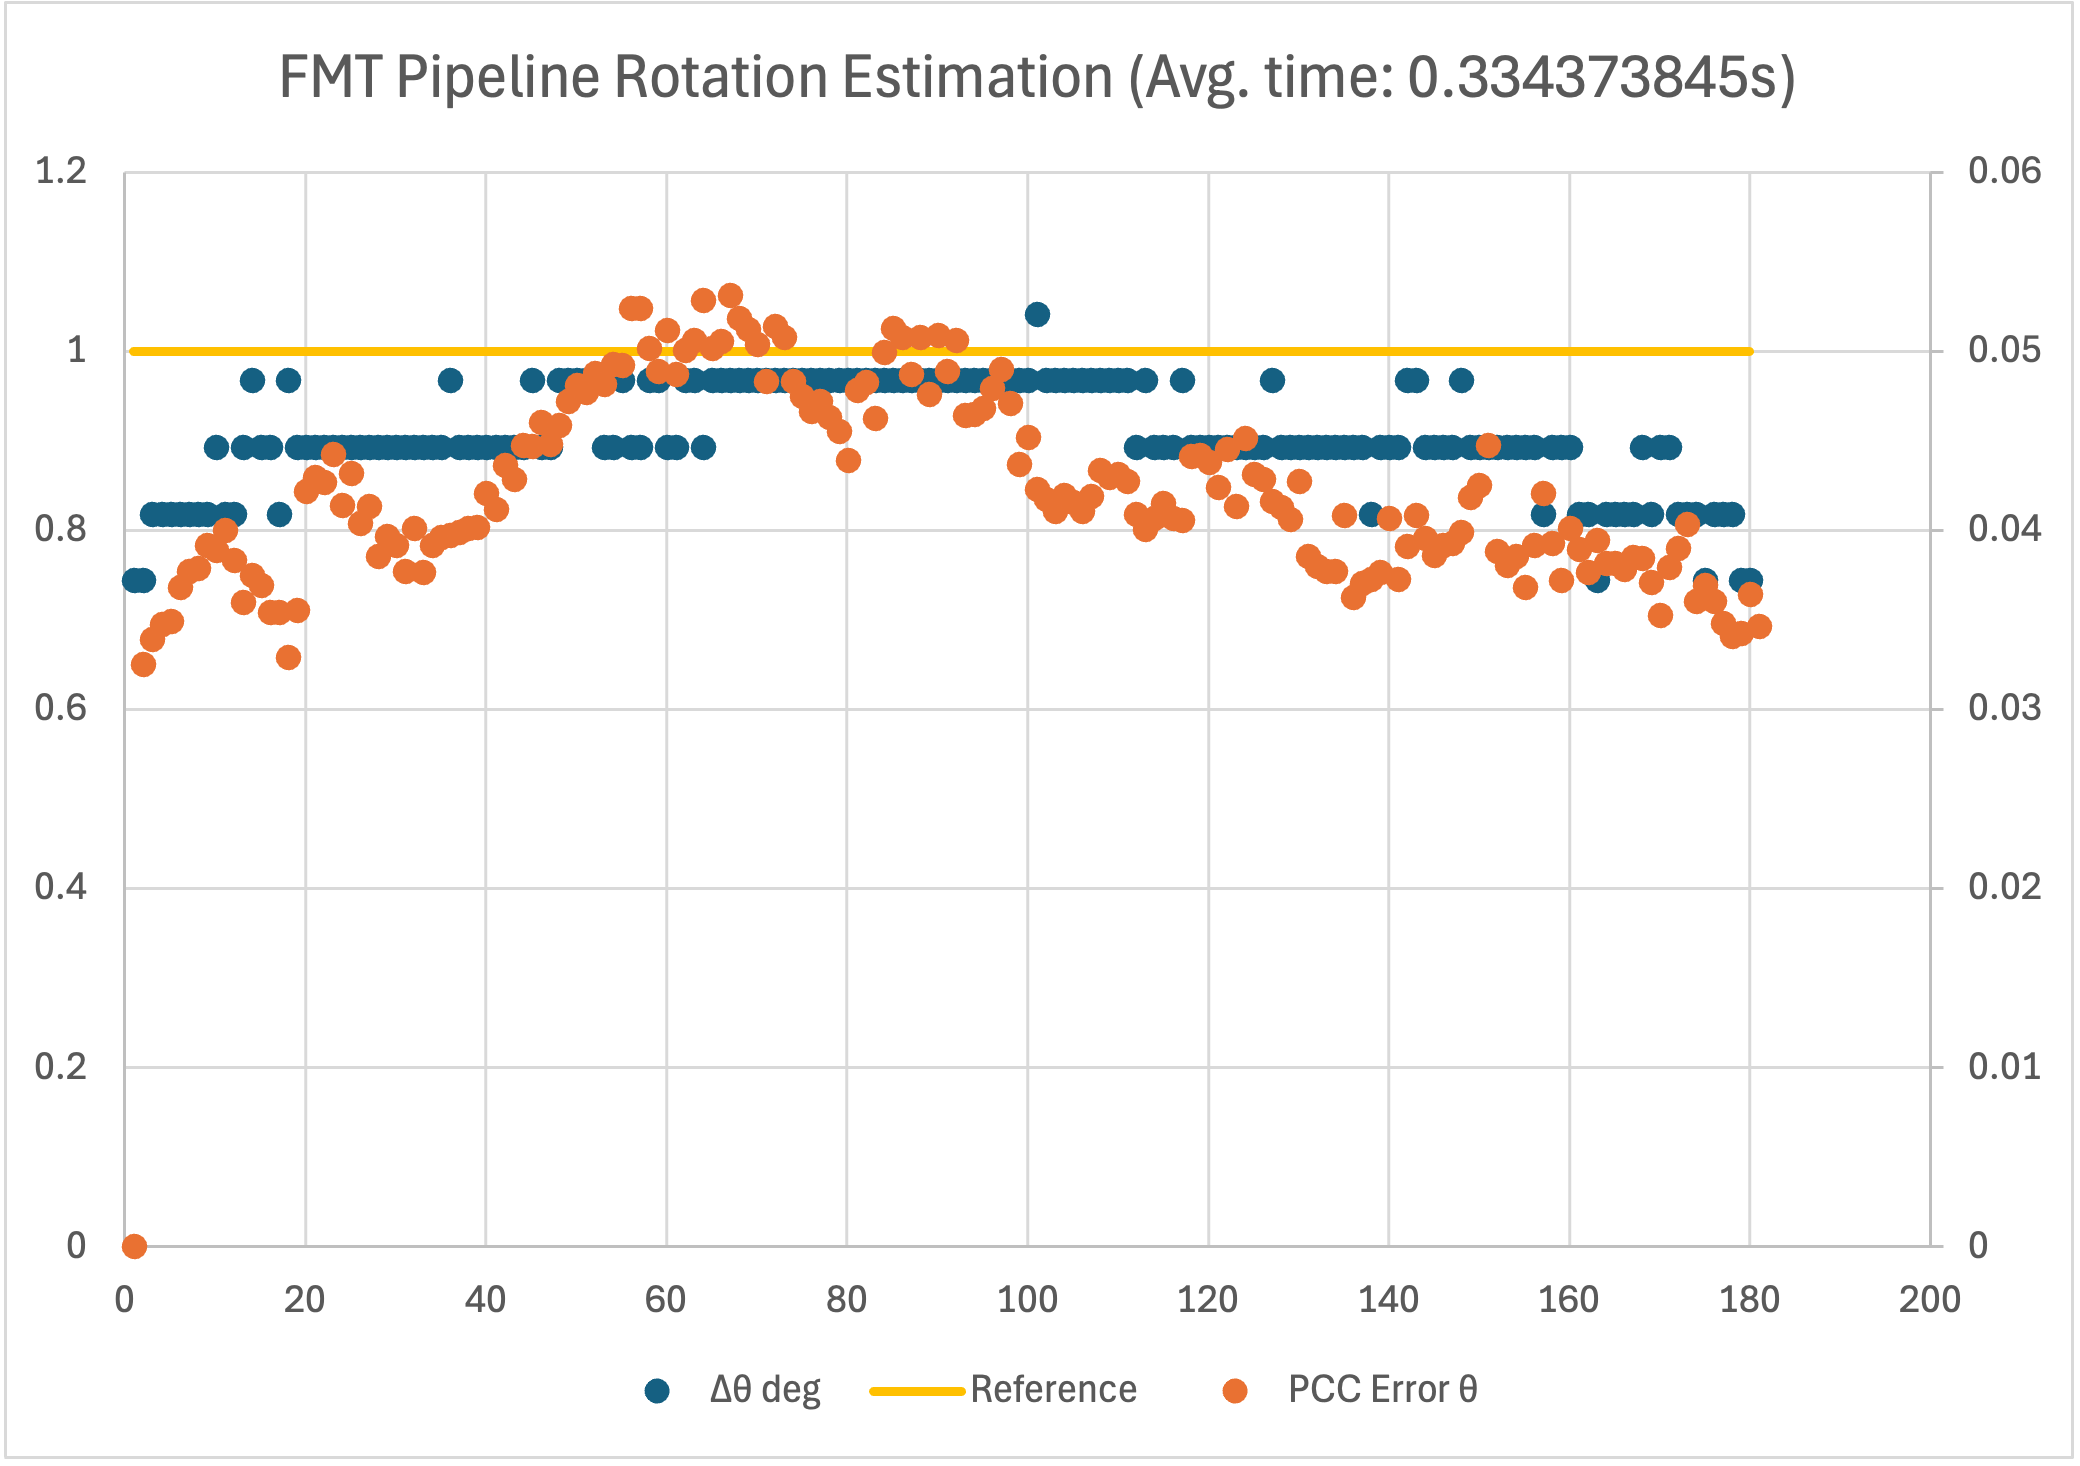
\includegraphics[width=.7\textwidth]{figures/results/rotation-skip-0/FMT-Rotation.png}
  \caption[Fourier-Mellin Pipeline Rotation Estimation Results]{Fourier-Mellin Pipeline Rotation Estimation Results}
  \label{fig:fmresults-skip-0}
\end{figure}


The FMT Pipeline struggled to estimate angles correctly at the beginning and the end of the test set frames. This coincides with frames that extend beyond the edge of the source image and are partially missing information. Counter-intuitively the registration error over these measurements is the lowest, showing a higher degree of confidence when compared to the measurements that were actually closes to the reference value. This is visible in the output \autoref{fig:fmcombined-skip-0}, which is sharpest in the middle where the registrations were closest to the true value, and blurry around the start and end of the semicircle.


\begin{figure}[H]
  \centering
  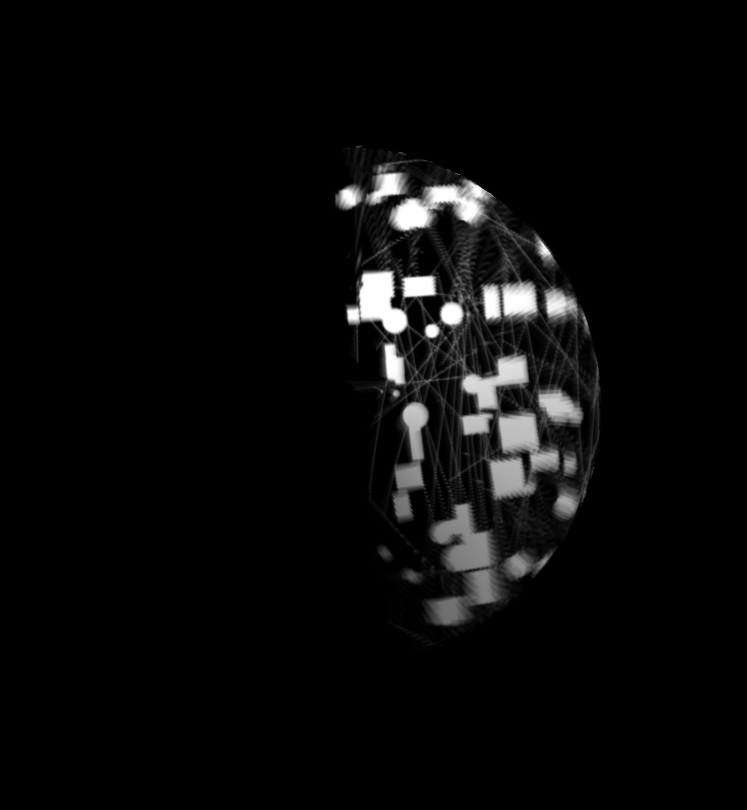
\includegraphics[width=.7\textwidth]{figures/results/rotation-skip-0/FMT.png}
  \caption[Fourier-Mellin Pipeline Rotation Estimation Mosaic]{Fourier-Mellin Pipeline Rotation Estimation Mosaic}
  \label{fig:fmcombined-skip-0}
\end{figure}

\begin{table}[H]
    \centering
    \begin{tabular}{|c|c|}
        \hline
        \textbf{Parameter} & \textbf{Spec} \\ \hline
        Sum of $\Delta\theta$ & 162.9669421º \\ \hline
        Average of $\Delta\theta$ & 0.905371901º \\ \hline
        StdDev of $\Delta\theta$ & 0.059270225º \\ \hline
        Min of $\Delta\theta$ & 0.743801653º \\ \hline
        Max of $\Delta\theta$ & 1.041322314º \\ \hline
        Average Error & 0.094628099º \\ \hline
        Average time & 0.334373845s \\ \hline
    \end{tabular}
    \caption{FMT Pipeline Results}
\end{table}



\begin{figure}[H]
    \centering
    \begin{subfigure}[b]{.45\textwidth}
        \centering
        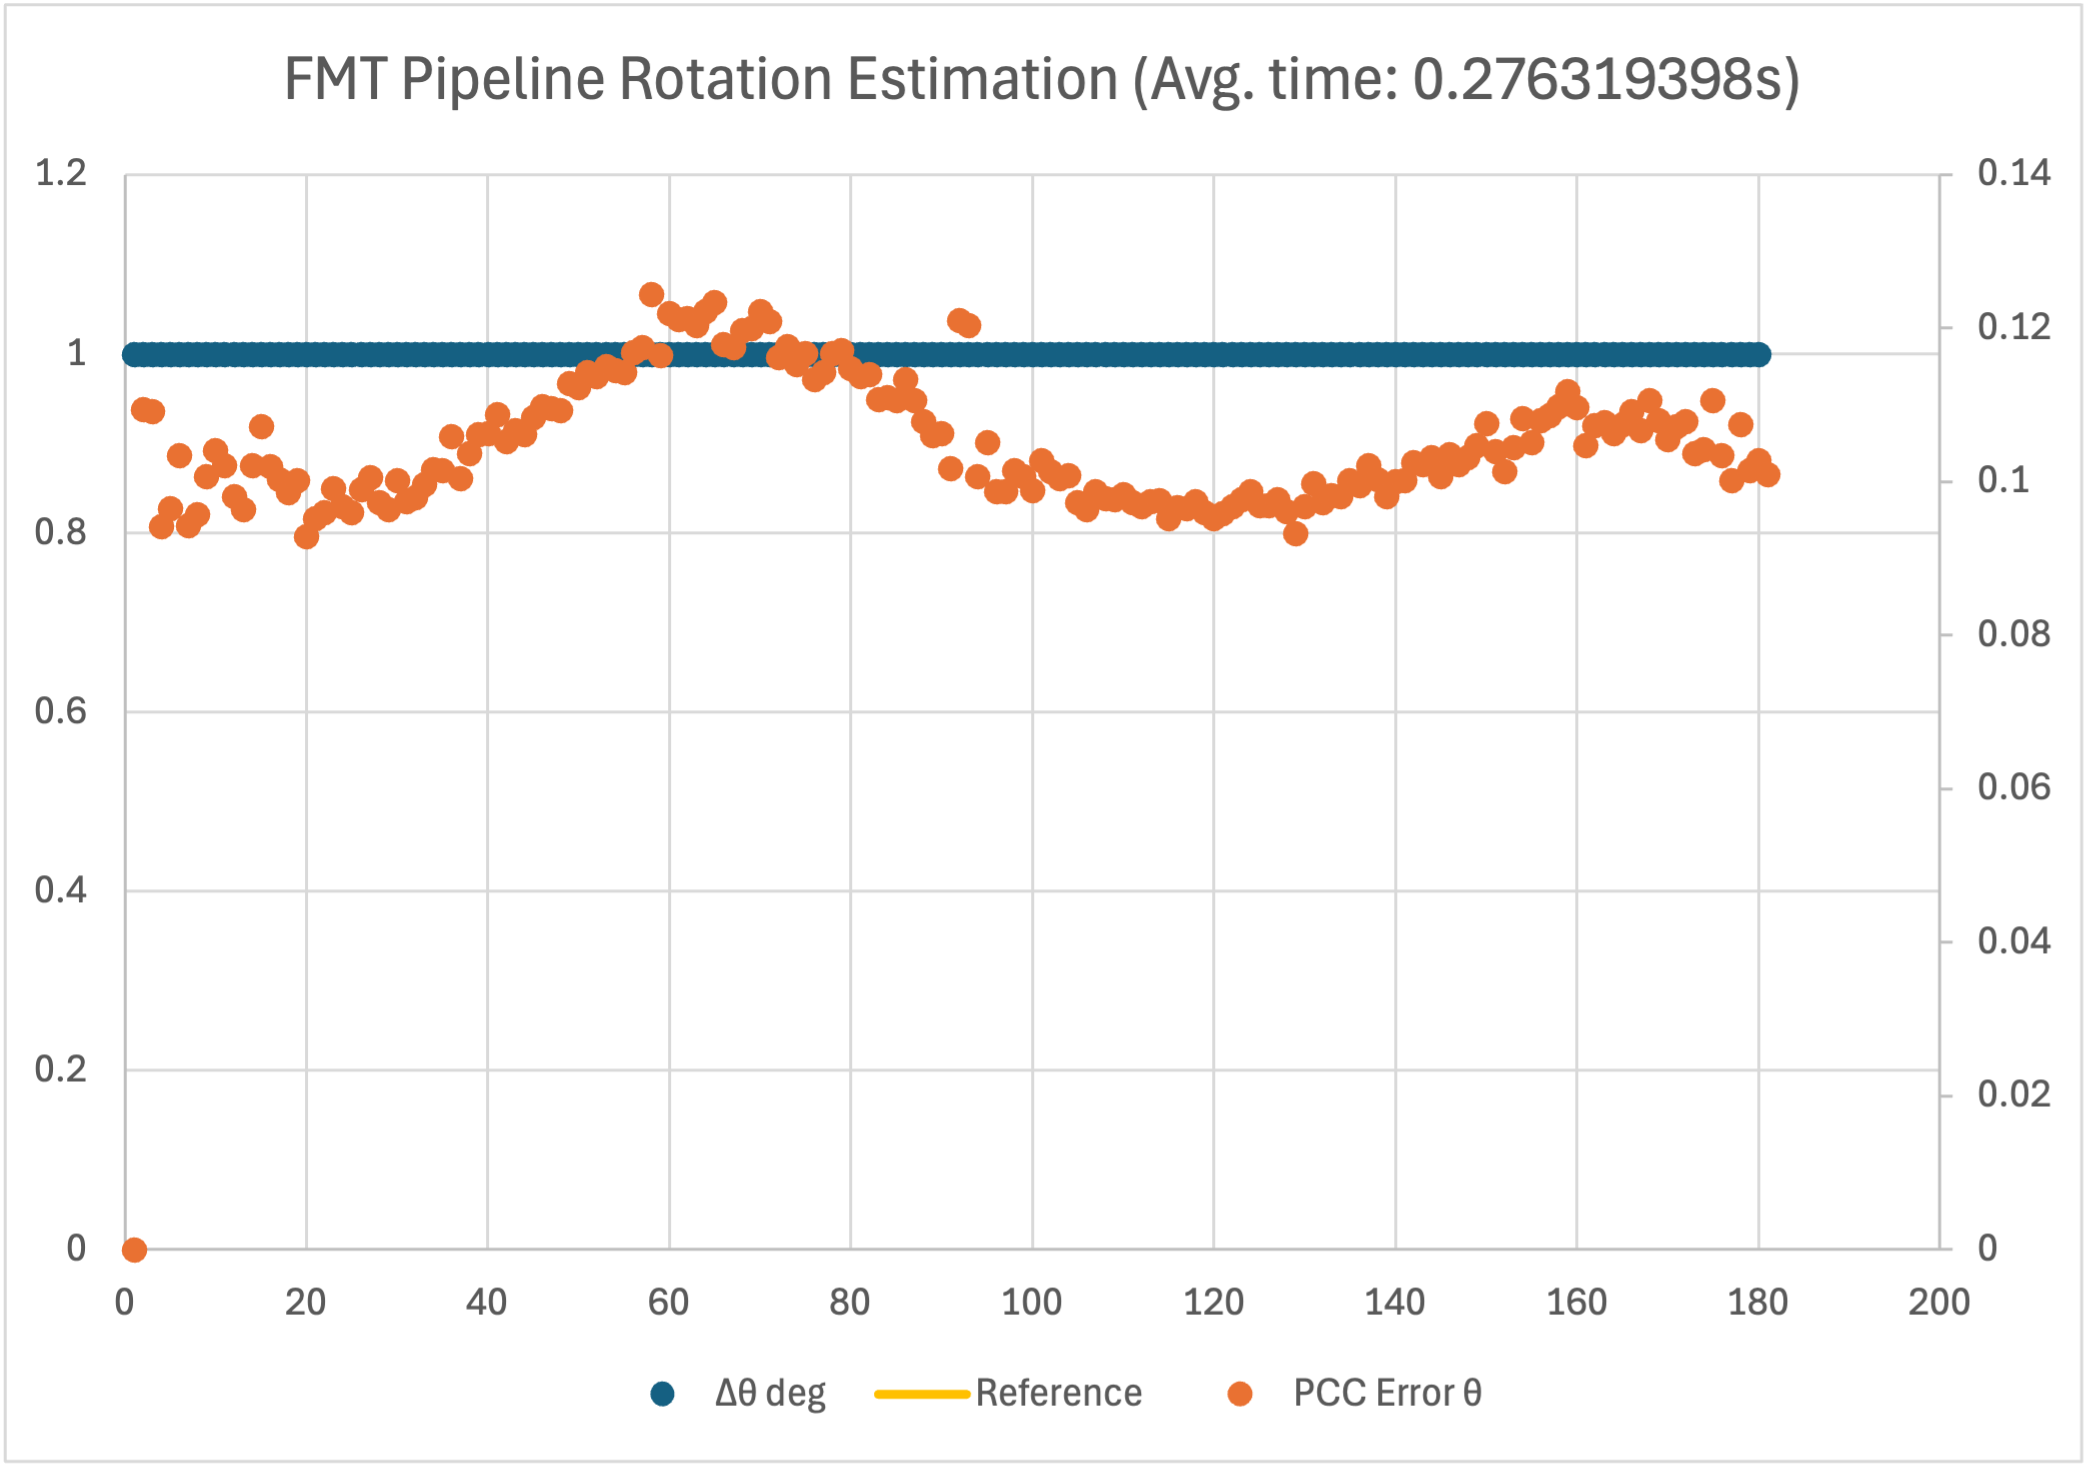
\includegraphics[width=\textwidth]{figures/results/rotation-skip-0/PC-Rotation.png}
        \caption{Rotation estimation}
        \label{sfig:pcrotation}
    \end{subfigure}
    \hfill
    \begin{subfigure}[b]{.45\textwidth}
        \centering
        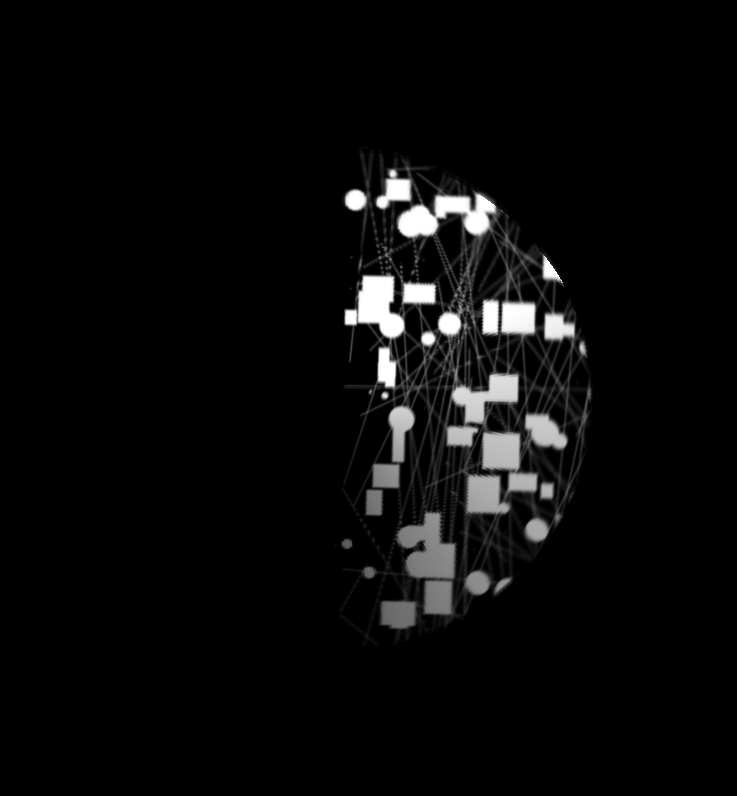
\includegraphics[width=\textwidth]{figures/results/rotation-skip-0/PC.png}
        \caption{Combined image}
        \label{sfig:pccombined-skip-0}
    \end{subfigure}
    \caption[\citeauthor{Hurtos2015} Pipeline Rotation Estimation Results]{Results from running the \citeauthor{Hurtos2015} Pipeline without skipping any frames in between.}
    \label{fig:subfig}
\end{figure}

\begin{table}[H]
    \centering
    \begin{tabular}{|c|c|}
        \hline
        \textbf{Parameter} & \textbf{Spec} \\ \hline
        Sum of $\Delta\theta$ & 180º \\ \hline
        Average of $\Delta\theta$ & 1 \\ \hline
        StdDev of $\Delta\theta$ & 0º \\ \hline
        Min of $\Delta\theta$ & 1º \\ \hline
        Max of $\Delta\theta$ & 1º \\ \hline
        Average Error & 0º \\ \hline
        Average time & 0.334373845s \\ \hline
    \end{tabular}
    \caption{FMT Pipeline Results}
\end{table}

\section{Translation estimation}

\section{Combined estimation}

\section{Effect of downsampling}
\chapter{Discussion}
\label{chap:discussion}

This chapter contains an assessment of the results and implementations, talking about some of the trade-offs as evidenced by the results\ref{chap:results}. It will also use this information to comment on what a more complete pipeline might look like. 

There are a couple of things to mention about the effect of resizing the image on registration speed:
\begin{itemize}
    \item The dip in the speedup on \autoref{fig:resizing-speedup} on \(R=0.75\) can be explained as the penalty incurred by adding the extra step of resizing the image.
    \item The speedup is more evident on the Fourier-Mellin Pipeline as it has extra modules that are affected by the frame size: Fourier Transform, and Log-Polar Transform. 
\end{itemize}

It was unexpected for the Fourier-Mellin Pipeline to outperform the \citeauthor{Hurtos2015}'s Pipeline in registration time. However, \autoref{fig:resizing-speedup} seems to suggest that given a small enough resizing ratio, the Fourier-Mellin Pipeline executes much faster. \citeauthor{Hurtos2015}'s claims don't take into account resizing, and in this case, their pipeline clearly outperforms \citeauthor{Reddy1996}'s Fourier-Mellin version.

On pure rotational movement, the \citeauthor{Hurtos2015}'s Pipeline performs so much better than the Fourier-Mellin Pipeline. This could be developed into an application of its own. If the sonar mosaic doesn't have to allow for translations, one could imagine a mode where the \acrshort{rov} rotates about its center and restricts translational movement. This would result in very accurate mosaics of the area around the drone. Another advantage of this approach is that this is closer to one of the cases for homography estimation with no caveats as mentioned in \autoref{sec:mosaicing}: rotation about the camera center. This assures no perturbations from shadows since they would always be in the same place. This allows us to get the best of both approaches.

Mosaicing has the side-effect of improving the resolution of the images. There are a couple of things that seem to affect this. First, parts of the image at a shorter range tend to have higher resolution. This is a side-effect of the Fan Transformation. At higher ranges the beams are farther apart which results in lower resolutions, but as they get closer to the source there is a higher concentration of data in a smaller area. Mosaicing lets us take advantage of both of these areas. Even at low resolution, averaging of the frames results in clearer images as they all contain "a little piece of the puzzle". The higher-resolution part of the image helps improve the resolution of the areas over which it passes as well. 

Although skipping frames could help in achieving real-time performance, mosaicing distant frames like in \autoref{fig:fmtranslationmosaic} could result in evident seams, which is not ideal. Choosing how many frames to skip should be tuned to the speed of the vehicle, and as seen in the results for translations in either axis, should aim to be less than 9 frames in between. The effect seems to be less on pure rotation as in \autoref{fig:pcmosaic}, where the seams are less noticeable. 

One of the main pitfalls of the Fourier-Mellin Pipeline when applied over sonar frames is the sheer number of transformations that are applied over it, and that it relies on working on images that have already undergone a Fan Transformation. This transformation is very lossy since every beam is compressed into a single origin point. A lot of usable data is lost in this overlap. On top of this, the rotation is estimated through too many steps: Fan Transformation $\rightarrow$ Fourier $\rightarrow$ Log-Polar Transform $\rightarrow$ Phase Correlation. It is evident that \citeauthor{Hurtos2015}'s approach is not only faster by performing Phase Correlation directly on the source image but also more accurate for small rotations/translations. 

Another disadvantage of the Fourier-Mellin approach is the Band-pass Filter pre-processing step, which introduces more parameters that must be tuned to achieve good performance. It is also present in the Raw Polar, but only for registering translations. On the Raw Polar Pipeline, tuning the Band-pass Filter has no effect on rotations. From this, it is evident that the Raw Polar Pipeline's approach to use the raw data for registering rotations is more robust than its Fourier-Mellin counterpart. Tuning the Band-pass Filter is a tough task as there is no obvious metric to choose when evaluating these parameters, since we lack the data to determine what the underlying signal in the frame actually is. 

On the other hand, one of the main pitfalls of the \citeauthor{Hurtos2015}'s pipeline is that it can't deal with distant rotations and translations as effectively as \citeauthor{Reddy1996}'s. This is a side-effect of running phase correlation over the raw frame, which is interpreted as a polar representation of the scene. While \citeauthor{Reddy1996}'s decouples rotations from translations by using the Fourier transform of the images, \citeauthor{Hurtos2015}'s applies phase correlation over the raw images. This is a smart optimization assuming very little translation between frames, but this approach will definitely struggle over not-so-closely aligned frames. As evidenced by \autoref{sec:sway-hurtos} and \autoref{sec:surge-hurtos}, the Raw Polar Pipeline is only good at registering surge translations, as it can't deal with pure sway. Rotations aren't decoupled from translations in the polar space, and so it turns out that translations along the sway axis (left and right) inflict the most change on the perceived rotation, affecting the overall registration. 

According to \citeauthor{Hurtos2015}\cite{Hurtos2015}:
\begin{quote}
    \textit{However, when working with the polar images, rotation is not decoupled from translational displacements, and shifts in Cartesian space create distortions in the polar domain. If the translational displacements are relatively small compared to the image’s size in each direction, the induced distortions in the polar image still allow for the recovery of the rotation by computing the shift in the angular direction.}
\end{quote}

It appears that they do not seem to realize that overall translational displacement is not the only metric to consider, but whether or not this translation is mostly on the surge or sway axis.

Another overlook on their part is the possibility of uneven spacing between beams according to the bearing table. This might currently be introducing some small error into the rotation estimation part of the pipeline. The uneven spacing is not taken into account by the algorithm currently, it only considers the \acrshort{fov}. 


Combining the strengths of both algorithms should be further explored, but given these results, they could be useful for adding global alignment to the process. So far, the described pipelines have focused on pair-wise registration of consecutive frames. According to \citeauthor{Hurtos2015}\cite{Hurtos2015} this open chain will lead to high cumulative error. To address this, \citeauthor{Hurtos2015}\cite{Hurtos2015} and \citeauthor{Das2021}\cite{Das2021} propose adding global alignment which involves attempting registration between non-consecutive frames that might be in the spatial or temporal vicinity of the current one, or using data from other sources, such as GPS, or in our case \acrshort{dvl} positioning. This data is merged with the original transformation chain using pose-based graphs. A pose graph, as proposed by \citeauthor{Kummerle2011}\cite{Kummerle2011} expresses positions as nodes and relative transformations as edges. As more edges are added, for example as the result of attempting global alignment the more information is available to try to minimize the error along the longer chains. A new combined pipeline might use \citeauthor{Hurtos2015}'s approach for incoming consecutive frames, but use the proposed adaptations to \citeauthor{Reddy1996}'s Fourier-Mellin Pipeline for global alignment against frames suspected to be in the vicinity.

On a separate note, it is interesting to see how the estimations seem to move in discrete steps, probably because increments in translation/rotation estimation are directly linked to pixel values, which are discrete themselves. In addition, down-sampling the image must decrease the number of discrete steps as it reduces the number of pixels. 

It is hard to evaluate the performance of the frames on real data, in particular, because it's hard to determine what the reference value should be. Rotations are easier because the pilot has more input about the heading and can control the drone to stay within certain ranges. Dimensions on features visible in the mosaics from \autoref{fig:sonar-mosaic} seem to be preserved even when the registration chain adds up to a bigger rotation than what was actually performed.
\chapter{Conclusion}
\label{chap:conclusion}

\section{Conclusion}

\section{Limitations}

\begin{itemize}
    \item No changes in depth.
    \item Scale not taken into account in either pipeline. Might be a measure of depth.
\end{itemize}


\section{Future work}

Using the Hurtos pipeline is good, however angle estimation is most likely wrong on real images because of the bearing table. This could be fixed by re-scaling the bearings axis so that all angles are evenly spaced. Additionally, it might be helpful to re-scale the range axis in the raw frames into log base so that scale might also be calculated through phase correlation. 

Ray supports pipelining operations to increase throughput. Currently each module has to finish before processing of the second module begins. In most cases, except in the Phase Correlation and the Mosaicing modules, the pipelines tends to be independent for each image. Using Ray for pipelining across modules might save some useful cycles.

GPU acceleration of the pipelines.


\chapter*{\bibname}
\printbibliography[heading=none]

% First paper

% \begin{paper}{papers/landes1951scrutiny.pdf}{paper:scrutiny}
%     Here, you may add a description of the paper, an illustration, or just give the bibliographic reference:
%     \begin{quote}
%         \fullcite{landes1951scrutiny}
%     \end{quote}
%     Or you may leave it empty, if you like.
% \end{paper}

% Second paper etc.

\appendix
\chapter{Additional Material}
\label{app:additional}

\section{Timing of modules}
\begin{table}[H]
    \centering
    \begin{tabular}{|c|c|c|c|c|}
        \hline
        Row Labels & Average of time & StdDev of time & Min of time & Max of time \\ \hline
        \verb|pipeline.Pipeline| & 0.334373845 & 0.195231211 & 0.268059969 & 2.845854044 \\ \hline
        \verb|pipeline.Pipeline_conditioning__1| & 0.106363857 & 0.180980164 & 0.084543943 & 2.523277044 \\ \hline
        \verb|pipeline.Pipeline_conditioning__1_FanModule2__1| & 0.079292439 & 0.007017289 & 0.073828936 & 0.129281044 \\ \hline
        \verb|pipeline.Pipeline_conditioning__1_PaddingModule__2| & 0.005277683 & 0.002123205 & 0.003836155 & 0.028264999 \\ \hline
        \verb|pipeline.Pipeline_conditioning__1_ResizeModule__0| & 0.02037254 & 0.179488065 & 0.00521493 & 2.414816856 \\ \hline
        \verb|pipeline.Pipeline_filtering__3| & 0.054460384 & 0.01186788 & 0.045929193 & 0.140566111 \\ \hline
        \verb|pipeline.Pipeline_filtering__3_BandpassModule__0| & 0.045252405 & 0.009429116 & 0.040208101 & 0.124923944 \\ \hline
        \verb|pipeline.Pipeline_filtering__3_MaskModule__1| & 0.006473091 & 0.004970803 & 0.004266977 & 0.047956944 \\ \hline
        \verb|pipeline.Pipeline_global_alignment__5| & 0.005665584 & 0.011317324 & 0.002096176 & 0.137736797 \\ \hline
        \verb|pipeline.Pipeline_global_alignment__5_UpdateTformModule__0| & 0.002116981 & 0.003729362 & 0.000874043 & 0.050754786 \\ \hline
        \verb|pipeline.Pipeline_IdentityModule__0| & 0.000410721 & 0.000265738 & 0.000173807 & 0.002635002 \\ \hline
        \verb|pipeline.Pipeline_IdentityModule__6| & 0.00103558 & 0.000510554 & 0.000609875 & 0.004172087 \\ \hline
        \verb|pipeline.Pipeline_MetricsModule__2| & 0.014786993 & 0.00506369 & 0.011919022 & 0.07575798 \\ \hline
        \verb|pipeline.Pipeline_OdometerModule__8| & 0.001772465 & 0.000973816 & 0.000936031 & 0.008838892 \\ \hline
        \verb|pipeline.Pipeline_pipeline.Pipeline__9| & 0.021402621 & 0.007335451 & 0.013242006 & 0.071824074 \\ \hline
        \verb|pipeline.Pipeline_registration__4| & 0.126420726 & 0.036122286 & 0.090725899 & 0.338999987 \\ \hline
        \verb|pipeline.Pipeline_registration__4_FourierModule__1| & 0.01765546 & 0.006538383 & 0.013945103 & 0.093924761 \\ \hline
        \verb|pipeline.Pipeline_registration__4_IdentityModule__0| & 0.001466208 & 0.000689269 & 0.000715017 & 0.004929066 \\ \hline
        \verb|pipeline.Pipeline_registration__4_IdentityModule__4| & 0.001474382 & 0.000815922 & 0.000459194 & 0.006044149 \\ \hline
        \verb|pipeline.Pipeline_registration__4_LogPolarModule__2| & 0.028288943 & 0.006598951 & 0.023254156 & 0.094389915 \\ \hline
        \verb|pipeline.Pipeline_registration__4_PhaseCorrelationModule__3| & 0.034928919 & 0.017288774 & 0.022396326 & 0.200668812 \\ \hline
        \verb|pipeline.Pipeline_registration__4_PhaseCorrelationModule__6| & 0.035303782 & 0.015808464 & 0.022093058 & 0.12102294 \\ \hline
        \verb|pipeline.Pipeline_registration__4_WarpModule__5| & 0.004428173 & 0.000915987 & 0.003745079 & 0.00955224 \\ \hline
        \verb|pipeline.Pipeline_WarpModule__0| & 0.020068741 & 0.007029614 & 0.012322903 & 0.069835663 \\ \hline
        \verb|pipeline.Pipeline_WarpModule__7| & 0.020182917 & 0.004524675 & 0.013231993 & 0.062887192 \\ \hline
        Grand Total & 0.044222309 & 0.096335889 & 0.000173807 & 2.845854044 \\ \hline
    \end{tabular}
    \caption{FMT Pipeline Timing Results}
\end{table}
\cleardoublepage
% \includepdf[pages=-]{appendices/NTNUProsjektavtale.pdf}

\end{document}
